%% LyX 2.4.0~RC3 created this file.  For more info, see https://www.lyx.org/.
%% Do not edit unless you really know what you are doing.
\documentclass[letterpaper,english]{article}
\usepackage[T1]{fontenc}
\usepackage[latin9]{inputenc}
\setlength{\parindent}{0pt}
\usepackage{color}
\usepackage{babel}
\usepackage{amsmath}
\usepackage{amssymb}
\usepackage{graphicx}
\usepackage[bookmarks=false,
 breaklinks=false,pdfborder={0 0 1},backref=false,colorlinks=true]
 {hyperref}
\hypersetup{
 allcolors=blue}

\makeatletter

%%%%%%%%%%%%%%%%%%%%%%%%%%%%%% LyX specific LaTeX commands.
\pdfpageheight\paperheight
\pdfpagewidth\paperwidth

%% Because html converters don't know tabularnewline
\providecommand{\tabularnewline}{\\}

%%%%%%%%%%%%%%%%%%%%%%%%%%%%%% User specified LaTeX commands.
\setlength{\parskip}{\medskipamount}

\usepackage{arxiv}
\usepackage{booktabs}
\usepackage{multirow}
\usepackage{xcolor}
\newcommand{\D}{\mathrm{\,d}}

\author{
\textbf{John C. Boik}\textsuperscript{1},
\textbf{Kobus Esterhuysen}\textsuperscript{1,6},
\textbf{Jacqueline B. Hynes}\textsuperscript{1,2},
\textbf{Axel Constant}\textsuperscript{3},\\
\textbf{Ines Hipolito}\textsuperscript{1,5},
\textbf{Mahault Albarracin}\textsuperscript{1,4},
\textbf{Alex B. Kiefer}\textsuperscript{1},
\textbf{Karl Friston}\textsuperscript{1,7}
}

\date{
\textsuperscript{1}VERSES, Los Angeles, CA, USA\\
\textsuperscript{2}Spatial Web Foundation, Los Angeles, CA, USA\\
\textsuperscript{3}Dept. of Engineering and Informatics, Univ. of Sussex, Brighton, UK\\
\textsuperscript{4}Institut Sante et societe, UQAM, Montreal, CAN\\
\textsuperscript{5}Macquarie University, Sydney, AUS\\
\textsuperscript{6}LearnableLoopAI.com, Custer, WA, USA\\
\textsuperscript{7}Queen Square Institute of Neurology, UCL, London, UK
}

\makeatother

\begin{document}
\title{EcoNet: Multiagent Planning and Control of Household Energy Resources
Using Active Inference}
\maketitle
\begin{abstract}
Advances in automated systems afford new opportunities for intelligent
management of energy at household, local area, and utility scales.
Home Energy Management Systems (HEMS) can play a role by optimizing
the schedule and use of household energy devices and resources. One
challenge is that the goals of a household can be complex and conflicting.
For example, a household might wish to reduce energy costs and grid-associated
greenhouse gas emissions, yet keep room temperatures comfortable.
Another challenge is that an intelligent HEMS agent must make decisions
under uncertainty. An agent must plan actions into the future, but
weather and solar generation forecasts, for example, provide inherently
uncertain estimates of future conditions. This paper introduces EcoNet,
a Bayesian approach to household and neighborhood energy management
that is based on active inference. The aim is to improve energy management
and coordination, while accommodating uncertainties and taking into
account potentially conditional and conflicting goals and preferences.
Unlike reinforcement learning approaches that require extensive training data
and lack principled uncertainty handling, or model predictive control methods
that assume deterministic dynamics, EcoNet leverages the free energy principle
to unify perception, learning, and action under a single objective.
A key technical contribution is the use of \emph{predictive transition
matrices} for exogenous state factors: rather than treating future outdoor
temperatures, occupancy, and electricity tariffs as static, each agent
updates its generative model's $B$ matrices at every time step using
available forecasts (weather predictions, published tariff schedules,
occupancy calendars). This allows the agent to anticipate environmental
changes within its planning horizon without requiring hand-crafted rules
or additional inference machinery.
Simulation results across four climate scenarios (5 seeds each)
demonstrate that the system achieves energy costs within 2\% of a
perfect-foresight Oracle on average, and up to 17\% below a
fixed-thermostat baseline lacking battery management, while
simultaneously reducing greenhouse gas emissions.
We further validate the approach across diverse climate conditions using
real weather data from four cities and two seasons, confirming robust
generalization without retraining, since active inference agents adapt
online through belief updating rather than offline gradient descent.
Beyond single-agent optimization, we investigate five coordination modes
of increasing sophistication: independent (static preferences), aligned
(dynamic context-dependent preferences), hierarchical (centralized
meta-agent), a novel Theory of Mind (ToM) mode based on
federated belief sharing \cite{friston2024federated}, and a
\emph{sophisticated} mode in which each agent maintains a phantom model
of the other agent's decision-making, enabling anticipatory cost-aware
planning.
In the ToM mode, agents share posterior beliefs rather than raw states,
enabling decentralized consensus formation through auditory likelihood
mappings in each agent's generative model. Across four synthetic climate
scenarios (5 seeds each), the Aligned mode achieves costs within 2\%
of a perfect-foresight Oracle on average, and the ToM+Belief mode
provides a further 3\% cost reduction in mild climates where the
thermostat has meaningful scheduling flexibility. Across real-weather
scenarios, both modes generalize without retraining, with cost savings
of 0.6\% aggregate. In the sophisticated mode, a cost-aware Thermostat Agent
uses a five-factor generative model that includes an energy demand state
driven by a phantom Battery Agent, while the Battery Agent maintains a
phantom Thermostat Agent for multi-step HVAC prediction. Combined with
predictive $B$ matrices and a 12-hour planning horizon, this architecture
enables principled cost--comfort trade-offs through the standard expected
free energy objective.
\end{abstract}
\keywords{Active Inference\and Home Energy Management Systems\and Distributed Energy Resources\and Multi-Agent Systems\and Bayesian Inference\and Smart Grid\and Theory of Mind\and Belief Sharing\and Predictive Transition Matrices}

\section{Introduction}

At any given moment, households and the utilities that supply them
with electricity face numerous choices regarding use and management
of their energy-related devices. Behind-the-meter devices can include
household heating, ventilation, and air conditioning (HVAC) systems
and distributed energy resources (DERs) such as solar panels and solar
and electric vehicle (EV) batteries. Utilities manage a wide assortment
of devices that also can include solar and battery systems. For example,
a utility might employ batteries to protect low-voltage transformers
\cite{RAOUFMOHAMED2021102975}.

The preferences for---and goals of---energy management can be conditional
and can conflict. A household might want to minimize energy costs,
yet wish to keep air conditioning systems on high during hot summer
afternoons, even during periods of peak energy costs, when time-of-use
(ToU) rates are high. A household might want to keep a room pleasantly
warm in winter, but only if the room is expected to be occupied, and
only if ToU rates are low. A utility might want to encourage home
charging of electric vehicle (EV) batteries, but to discourage large
numbers of households from doing so at the same moment. As a last
example, a household might want to charge a solar battery while the
sun is shining or ToU rates are low, but discharge when rates are
high. To ensure the battery has adequate charge to serve household
needs during high ToU periods, the household might need to track weather
forecasts and plan ahead, perhaps many hours in advance.

Intelligent energy management that adapts to custom goals and preferences
is important for comfort, safety, cost, and environmental impact,
including impacts related to energy-associated greenhouse gas emissions.
DER penetration is increasing \cite{osti_1784528}, in part due to
climate change concerns, and as it does there is growing need to coordinate
energy use and generation, not just within a household but also within
neighborhoods and distribution regions. As just one example of the
challenges, high penetration of uncoordinated rooftop solar can reduce
the reliability of distribution grids \cite{denholm2024maintaining}.

This paper introduces EcoNet, a Bayesian approach to household and
neighborhood energy management based on active inference \cite{SMITH2022102632}.
The EcoNet project aims to improve energy management and coordination,
while taking into account potentially conditional and conflicting
goals and preferences, and accommodating inherent uncertainties associated
with, for example, forecasts of weather, room occupancy, and energy
use and generation.

A key distinction from existing approaches is that active inference provides
a single principled framework that naturally integrates planning under uncertainty,
online model learning, and multi-objective optimization. Reinforcement learning
(RL) methods require extensive offline training, lack built-in uncertainty
quantification, and struggle with conditional constraints that change over time
(e.g., preferences that depend on occupancy or ToU period). Model predictive
control (MPC) assumes access to an accurate deterministic model and does not
natively support online parameter learning or exploration. In contrast, EcoNet's
active inference agents maintain probabilistic beliefs over hidden states,
learn transition dynamics from data via Dirichlet concentration updates, and
select actions by minimizing expected free energy---a quantity that automatically
balances goal-seeking (exploitation) with uncertainty reduction (exploration).
Furthermore, the preference structure of active inference agents can be made
context-dependent (e.g., the Battery Agent's preferences shift between charging
and discharging based on the current ToU period), providing a principled mechanism
for handling conditional goals that would require ad hoc reward shaping in RL.

In general, conflicting goals can arise from many sources, including
the directive to conform to norms---legal, ethical, and cultural---which
themselves can conflict. In this sense, the EcoNet project addresses
artificial intelligence (AI) governance \cite{Dhaou-2024}, understood
as the mitigation of risks posed by AI systems. One such risk is the
failure of an artificial agent to comply with the complex knitting
of human-defined legal, ethical and cultural norms that underlies
human social coordination \cite{Constant-2025,Constant2025Path,Constant2024-ev}.

Here we present a proof-of-concept model that involves energy
management in a single one-room household. The managed devices are
a HVAC system, a solar panel, and a battery that can be charged by
the grid or by solar. Devices are controlled by two agents. The discrete
actions available to the \textit{Thermostat Agent} are to set the
thermostat to \textit{cool}, \textit{heat}, or \textit{off}. The actions
available to the \textit{Battery Agent} are to set the battery to
\textit{charge}, \textit{discharge}, or \textit{off}. The household
prefers to minimize energy costs and grid-associated greenhouse gas
emissions, while preferences for room temperature are conditional
on ToU rates and expected room occupancy. By use of a multi-agent
approach, we set the stage for coordination in more complex settings,
such as between households and over larger regions. We demonstrate
that EcoNet achieves lower energy costs and greenhouse gas emissions
than both unmanaged and rule-based baselines, generalizes across
diverse climates without retraining, and can learn thermodynamic
parameters online. We further investigate five coordination modes
(independent, aligned, hierarchical, Theory of Mind with belief sharing,
and sophisticated mutual inference with predictive transition matrices),
showing how agents that share posterior beliefs or maintain phantom
models of each other can achieve superior performance across cost,
comfort, and emissions through decentralized coordination
\cite{friston2024federated,vasil2020world}.

The following sections discuss related work, provide an overview of
active inference, describe the EcoNet model including a novel
belief-sharing architecture for inter-agent coordination, present
simulation results including baseline comparisons, climate sensitivity
analyses, and a five-mode coordination study, and discuss outcomes
and future work.

\section{Related Work}

Given the importance of distributed energy resources and stresses
on energy grids from increased electrification, a large body of research
addresses utility options related to DERs and energy use, including
utility-level control of or incentives for DER management \cite{smith-2024,Kurella31122025}.
Public datasets of household energy use and grid dynamics are available
to assist researchers \cite{Altamimi-2024,OEDI_Dataset_2981,NEEA_Org}.
From a utility perspective, households and commercial buildings can
offer flexibility services such as energy generation, load shifting,
and peak shaving, as well as ancillary services to help maintain grid
stability and function. These services include primary frequency response,
active power smoothing, exchange of reactive power for voltage regulation,
contributions to fault clearing, and voltage harmonic mitigation \cite{Demoulias-2020}.
Such capacities are of obvious interest to policymakers, planners,
manufacturers, consumer groups, and other stakeholders in energy and
environmental domains.

Utility programs that encourage households to offer flexibility and
ancillary services are typically implemented using price signals,
such as ToU rates, or other kinds of incentives. While price-based
programs empower prosumers and maintain privacy relative to direct
utility control of household devices, they depend on consumer attention
and action for success. Utilities thus benefit when households employ
Home Energy Management Systems (HEMS) for intelligent, automated or
semi-automated control of energy devices. Households benefit also,
as use of HEMS tends to reduce energy costs and increase comfort (e.g.,
via temperature control), among other benefits \cite{Mahapatra2022-zp}.

\subsection{RL and MPC for Home Energy Management Systems}

A sizable body of work addresses DER and energy management by HEMS
or related systems that serve building clusters or other localized
aggregations \cite{Zafar,Mahapatra2022-zp}. Households, neighborhoods,
and building clusters are the current focus of EcoNet.

Reinforcement learning (RL) is a family of methods in which an agent learns
a control policy by interacting with an environment and receiving scalar
reward signals. The agent seeks to maximize cumulative expected reward over
time, typically using value function approximation or policy gradient
methods. RL does not require an explicit model of the environment, which
makes it flexible but also data-hungry, as the agent must explore extensively
to discover good policies.

Mason and Grijalva describe a reinforcement learning model applied
to building energy management \cite{mason2019review}. Wu et al. discuss
a deep-RL HEMS that uses intrusive load monitoring to recognize and
categorize human activity, the results of which are used to make energy-related
decisions \cite{WU2024114951}. Yu et al. describe a deep RL multi-agent
model that minimizes energy costs of HVAC systems in commercial buildings
\cite{yu2020multiagentdeepreinforcementlearning}. Touzani et al.
develop a deep RL approach for integrated control of HVAC and solar
battery storage and test it in a physical building against rule-based
strategies \cite{TOUZANI2021117733}. A variety of other groups have
studied RL frameworks for energy trading, demand response, load shedding,
voltage control, and microgrid dispatch \cite{shojaeighadikolaei2022distributed,shengren2023optimal,zhang2023deep,chen2022reinforcement,Ye-2023}.

Model predictive control (MPC) is an optimization-based approach that uses an
explicit model of the system to predict future behavior over a finite horizon.
At each time step, MPC solves a constrained optimization problem to determine
the control inputs that minimize a cost function, applies the first input,
and then re-solves at the next step with updated state information
\cite{Schwenzer2021-bl}. Khabbazi
et al. review 24 field demonstrations of MPC and RL for HVAC control
in residential buildings and 80 in commercial buildings \cite{khabbazi2025}.
They report that average cost savings are 16 percent for residential
buildings and 13 percent for commercial buildings. Hartel and Bocklisch
compare RL and MPC systems for minimizing energy costs of solar battery
systems \cite{Hartel-2023}. Wang et al. compare several RL algorithms
against MPC and rule-based systems for heat pump control \cite{WANG2023120430}.

Despite their potential benefits neither MPC nor RL have seen wide
adoption in DER/energy management \cite{khabbazi2025}. Wang and Hong
identify three barriers for RL: 1) time-consuming and data-intensive
training requirements; 2) security and robustness concerns (regarding
the potential for detrimental or catastrophic decision making); and
3) lack of generalizability, where each new implementation requires
new training \cite{WANG2020115036}. A barrier for MPC is that it
requires a reasonably accurate model of the system and environment,
which is not always available, and which can change over time if devices
or patterns of management change.

Nweye et al. address the three RL barriers in their model of a 17-building
grid-interactive residential community \cite{NWEYE2023121323}. The
aim is to minimize energy consumption and cost, minimize emissions,
and provide grid flexibility services. To reduce data requirements
they implement digital twins of real buildings, constructed in the
CityLearn gymnasium \cite{Vazquez-2019}. They address security and
comfort via an occupancy-aware RL control architecture. And they address
generalizability through use of transfer learning.

In their system, the first step is to obtain a history of energy-related
data from real buildings. The second step is validation of the simulation
environment and control agent. Following validation, experiments are
carried out to determine what control policy has the best performance.
A best-performing control policy for a building is one that yields
the best outcome for a set of KPIs. Finally, the best-performing control
policies are deployed in the real-world grid-interactive community
in the respective building whose data they were trained on, or are
used as source for transfer learning and leveraged in other target
buildings.

In addition to the RL and MPC barriers already mentioned, DER systems
and environments can exhibit substantial uncertainty. Forecasts for
weather and solar generation can be inaccurate, for example. Conventional
RL and MPC models are not probabilistic, however, and so are not well
equipped to handle uncertainty. To address uncertainty quantification,
Zhang et al. develop a Bayesian deep RL control approach for microgrids
in which they replace the deterministic neural network in traditional
RL with a Bayesian probabilistic one \cite{zhang-202310005226}.

\subsection{Active Inference for Home Energy Management Systems}

In contrast to conventional RL and MPC, active inference employs a
generative probabilistic model that naturally accounts for uncertainty.
Like MPC, active inference requires a model, although that model can
be readily learned from data, especially if the model structure is
known. Unlike RL, active inference models are not usually data intensive,
and conditional constraints on behavior can be easily implemented.
Also unlike RL, a method for balancing agent exploration and exploitation
stems from first principles \cite{tschantz2020reinforcementlearningactiveinference}.
Furthermore, active inference is apt for multiple constraint satisfaction
problems, by specifying preferences in terms of probability distributions
over outcomes. Active inference is particularly useful when an agent
must plan ahead and can act to reduce uncertainty. For these reasons,
active inference offers an attractive approach for DER and energy
management. However, the study of active inference in this domain
is very new.

To the best of our knowledge, only a few studies exist on the topic.
Albarracin et al. have explored the use of active inference in sustainability and
resource management more generally \cite{albarracin2024sustainability,albarracin2024modeling}.
Specific to HEMS, Nazemi et al. propose a dual-layer, hybrid active
inference architecture for tackling both building- and community-level
energy management \cite{danial2025active}. The bottom layer is a
continuous state-space model of building energy use, where HVAC systems
are controlled. The top layer (termed \textit{community manager})
is a discrete state-space model of aggregated energy use over buildings,
with the aim to keep power consumption within the proximity of day-ahead
plans. The community manager controls a shared energy storage system,
distributed renewables, and market transactions in response to external
price signals. Linking the two layers is a privacy-preserving interaction
protocol. In simulations, each building is represented by a digital
twin, an EnergyPlus model \cite{CRAWLEY2001319}, that integrates
real-time factors such as energy use, PV generation, energy storage,
and occupancy schedules.

The authors benchmark model performance against optimal planning (in
the fully observable case) and against RL approaches in which the
RL model is trained on a history of observables for the buildings
in question. Compared to RL models, the active inference agent predicts
indoor room temperatures that align more closely with desired temperatures.
This is not surprising, perhaps, as the active inference model encapsulates
prior knowledge about the HVAC and other systems. The community manager
successfully optimizes battery usage and market transactions, even
under an extreme pricing scenario.

Active inference applied to DER and energy management is new and promising,
potentially offering robust, uncertainty-aware coordination among
intelligent agents in a household and between households. Below, we
explore a multi-agent system in a single household. The present work extends
our earlier proof-of-concept by introducing baseline comparisons against
unmanaged and rule-based controllers, climate sensitivity analysis using
real weather data from four geographically diverse cities, extended
simulation horizons, and formal validation of physical constraints.
But before describing
that model, we provide background on active inference.

\section{Active Inference}

Active inference originated within the neuroscience field to explain
how agents perceive, learn, and act in uncertain environments. It
is a Bayesian model-based approach that considers perception, (parameter)
learning, and action as intertwined processes of inference \cite{friston2017graphical,millidge2020relationship,SMITH2022102632}.
Inference is achieved by minimizing free energy via variational inference.
As a brief primer, for data $x$ and a parameter $\theta$ treated
as a random variable, Bayes theorem (see \cite{bishop2006} for a
comprehensive treatment) is

\begin{equation}
p(\theta|x)=\frac{p(\theta,x)}{p(x)}=\frac{p(x\mid\theta)\,p(\theta)}{\int p(x\mid\theta)\,p(\theta)\D\theta}\,,\label{eq:bayes}
\end{equation}

where the marginal likelihood $p(x)$ is called the \textit{model
evidence}. The right-hand side of Equation~\ref{eq:bayes} is the \textit{likelihood} times \textit{prior,
$p(\theta)$,} divided by the evidence. The left-hand side is the
\textit{posterior,} which is the updated prior after seeing the data.
Maximum Likelihood Estimation II (also called empirical Bayes or
evidence maximization; see \cite{bishop2006}) estimates $\theta$ by
maximizing the model evidence:

\begin{equation}
p(x)=\int p(x\mid\theta)\,p(\theta)\D\theta\,.\label{eq:mle2}
\end{equation}

Commonly, this integral is intractable. Progress is made by maximizing
a lower bound called the \textit{variational lower bound} or \textit{evidence
lower bound} (ELBO). It can be derived by choosing a distribution
$q(\theta)$ that is similar to but simpler than $p(\theta\mid x)$,
and that is introduced independently of the data $x$ but is
subsequently optimized to approximate $p(\theta \mid x)$. Using Jensen's inequality
(see \cite{bishop2006,cover2006}) and after a series of manipulations, the result is

\begin{align}
\ln p(x) & \geq\mathbb{E}_{q}\left[\ln\frac{p(\theta,x)}{q(\theta)}\right]\nonumber \\
 & =\mathbb{E}_{q}\left[\ln p(\theta,x)\right]+H(\theta)\,,\label{eq:Jensen}
\end{align}

where the right-hand sides are called the ELBO, $H$ is entropy, and
the negative ELBO is called \textit{free energy:}
\begin{align}
F(\theta) & =\mathbb{E}_{q}\left[\ln q(\theta)\right]-\mathbb{E}_{q}\left[\ln p(\theta,x)\right]\label{eq:FE}\\
 & \geq-\ln p(x)\,.\nonumber
\end{align}
The right-hand side of the last line in Equation~\ref{eq:FE} is called \textit{surprisal}.
Thus, minimizing free energy is equivalent to estimating the posterior
by minimizing an upper bound on surprisal.

By minimizing free energy, agents implicitly infer the hidden causes
of their sensory inputs and select actions that fulfill their goals
or objectives. In short, active inference unifies perception, learning,
and action selection under a single mathematical principle.

An active inference agent possesses (or is) a generative model of
its environment that predicts sensory inputs and the consequences
of actions. The agent updates its beliefs about the world in response
to observations and chooses actions that minimize expected free energy,
balancing exploration (reducing uncertainty) and exploitation (achieving
goals). The environment, in contrast, is a generative process that
reacts to agent actions, generating potentially noisy observations
that the agent must account for. Commonly, the agent is constructed
as a discrete, partially observed Markov decision process (POMDP),
although continuous state-space models are possible \cite{Wade-2021,Catal-2020,collis2024learninghybridactiveinference}.
Deep learning has also been explored in this setting as deep active
inference \cite{Ueltzhoffer2018,tschantz2019scalingactiveinference,champion2023deconstructingdeepactiveinference}.

In each time step of a simulation, an agent typically performs perception,
learning, policy evaluation, and action selection. Perception entails
inferring hidden states of the generative model based on potentially
noisy observations obtained from the environment. Learning involves
updating the parameters of the generative model to better explain
observed data. In policy evaluation, the expected free energy (EFE)
of each policy available to the agent is calculated. A policy is a
series of potential actions over a rolling horizon of a specified
length. Alternatively, marginal EFE over the next action can be calculated.
Action selection involves choosing a policy (or action) based on its
EFE. The selected action (e.g., the first action in a selected policy)
is then communicated to, and affects, the environment.

The core of active inference is a joint generative model,

\begin{equation}
p(\tilde{o},\tilde{s},\pi)\,,\label{eq:generative_model}
\end{equation}

where $o$ signifies observations; $s$ signifies states (beliefs
about hidden or latent states); the tilde accent signifies a series
of sequential values over a simulation, from time $t_{1}$ to $t_{T}$;
and $\pi$ signifies the policy that is chosen in each time step,
with each policy being a series of sequential actions over a policy
length, $\tau$.

The expected free energy is evaluated under a posterior predictive
density, $\bar{q}$, over observations in the future, conditioned
on a particular policy (with prior preferences or constraints usually
denoted by \textit{C}). The EFE is derived as follows: two variational
distributions are employed during simulation, both using the mean-field
approximation shown by terms to the right of the arrows:

\begin{align}
q(\tilde{s},\pi) & =q(\pi)q(\tilde{s}\mid\pi)\rightarrow q(\pi)\prod_{\tau}q(s_{\tau}\mid\pi)\label{eq:variational1}\\
\bar{q}(\tilde{o},\tilde{s},\pi) & =q(\pi)q(\tilde{o},\tilde{s}\mid\pi)\rightarrow q(\pi)\prod_{\tau}q(o_{\tau},s_{\tau}\mid\pi)\,.\label{eq:variational2}
\end{align}

The factorized distributions in Equations~\ref{eq:variational1}--\ref{eq:variational2} and the generative model (Equation~\ref{eq:generative_model}) can be substituted
into Equation~\ref{eq:FE} to obtain the free energy for a particular
policy in a particular simulation step:

\begin{align}
F & =-\mathbb{E}_{q(\tilde{s}\mid\pi)}\left[\ln\frac{p(\tilde{o},\tilde{s}\mid\pi)\,p(\pi)}{q(\tilde{s}\mid\pi)\,q(\pi)}\right]\label{eq:F_policy}\\
 & =-\mathbb{E}_{q(\tilde{s}\mid\pi)}\left[\ln\frac{p(\tilde{o},\tilde{s}\mid\pi)}{q(\tilde{s}\mid\pi)}\right]+D_{\mathrm{KL}}\left[q(\pi)\parallel p(\pi)\right]\nonumber \\
 & =\mathbb{E}_{q(\pi)}\left[F_{\pi}\right]+D_{\mathrm{KL}}\left[q(\pi)\parallel p(\pi)\right]\nonumber \\
F_{\pi} & =-\mathbb{E}_{q(\tilde{s}\mid\pi)}\left[\ln\frac{p(\tilde{o},\tilde{s}\mid\pi)}{q(\tilde{s}\mid\pi)}\right]\,.\nonumber
\end{align}

To minimize $F$ in Equation~\ref{eq:F_policy}, we take its derivative with respect to $q(\pi)$
and set it to zero, resulting in

\begin{align}
q_{0}(\pi) & =\sigma\left(\ln p(\pi)-G_{\pi}\right)\label{eq:policy_posterior}\\
G_{\pi} & =-\mathbb{E}_{q(\tilde{o},\tilde{s}\mid\pi)}\left[\ln\frac{p(\tilde{o},\tilde{s}\mid\pi)}{q(\tilde{s}\mid\pi)}\right]\,,\label{eq:EFE}
\end{align}

where $q_{0}$ is the belief prior to observations, $\sigma$ is the
softmax function, and the negative expected free energy, $G_{\pi}$,
is a sum over each step of a policy. The distribution $\bar{q}$ is
substituted for $q$ when taking expectations of free energy in
Equation~\ref{eq:EFE} to finesse a shortcoming that would otherwise
occur. With $q$ rather than $\bar{q}$, $q_{0}$ would not accommodate
our prior knowledge that outcomes will become available in the future
\cite{parr2019}. With $\bar{q}$, future (not yet seen) observations
enter the expectations as random variables. In each simulation step
the agent selects the policy that it expects will lead to the lowest
free energy.

Dropping the accents, the negative expected free energy of a policy
step can be decomposed as

\begin{align}
G_{\pi} & =-\mathbb{E}_{q(o,s\mid\pi)}\left[\ln\frac{p(o,s\mid\pi)}{q(s\mid\pi)}\right]\nonumber \\
 & =\underset{\mathit{risk}}{\underbrace{D_{\mathrm{KL}}\left[q(o\mid\pi)\parallel p(o\mid C)\right]}}+\underset{\mathit{ambiguity}}{\underbrace{\mathbb{E}_{q(s\mid\pi)}\left[H(p(o\mid s)\right]}}\label{eq:EFE_decomp}\\
 & =-\underset{\mathit{information\,gain}}{\underbrace{\mathbb{E}_{q(o,s\mid\pi)}\left[\ln\frac{q(s\mid o,\pi)}{q(s\mid\pi)}\right]}}-\underset{\mathit{expected\,utility}}{\underbrace{\mathbb{E}_{q(o\mid\pi)}\left[\ln p(o\mid C)\right]}\,,}\nonumber
\end{align}

where $p(o\mid\pi)$ has been replaced with $p(o\mid C)$, where $C$
is a vector of preferences. Thus, as shown in Equation~\ref{eq:EFE_decomp}, the agent selects actions that fulfill
goals (i.e., maximize expected utility) and that reduce uncertainty
(i.e., maximize information gain).

\section{Model Description}

Our HEMS model consists of two heterogeneous agents in a one-room
building. The energy-related devices are a HVAC system, a solar panel,
and a battery that can be charged by the grid or by solar. The building
also has a baseline pattern of energy use over the course of a day
(e.g. peak energy use in the morning and evening) that is not controllable.
The Thermostat Agent controls the thermostat, with discrete actions
of \textit{cool}, \textit{heat}, or \textit{off}. Its preference is
to keep the room at a comfortable temperature, conditional on occupancy
and ToU rate. If the room is expected to be unoccupied, a lower temperature
is preferred.

The Battery Agent controls the battery, with discrete actions of \textit{charge},
\textit{discharge}, and \textit{off}. Its preference is to minimize
total household energy costs and grid-associated greenhouse gas emissions.
Thus, not only do the two agents control different devices and consist
of different generative models, they potentially exhibit conflicting
preferences: a warm room, for the Thermostat Agent, and low energy
cost, for the Battery Agent.

The input data consists of a table of time series, based on two-hour
steps. Variables are time of day, solar generation, baseline load,
ToU rate, outdoor temperature, room occupancy, and greenhouse gas
emission rate. All values are synthetic, but are meant to reflect
semi-realistic conditions. Tracking and controlling the temperature,
energy use, solar generation, and other processes in a real building
is not the purpose of this study. Rather, the purpose is to demonstrate
proof of concept. A pseudo-factor graph depicting the model is provided
in Figure \ref{fig:factor=000020graph}.

\begin{figure}
\begin{centering}
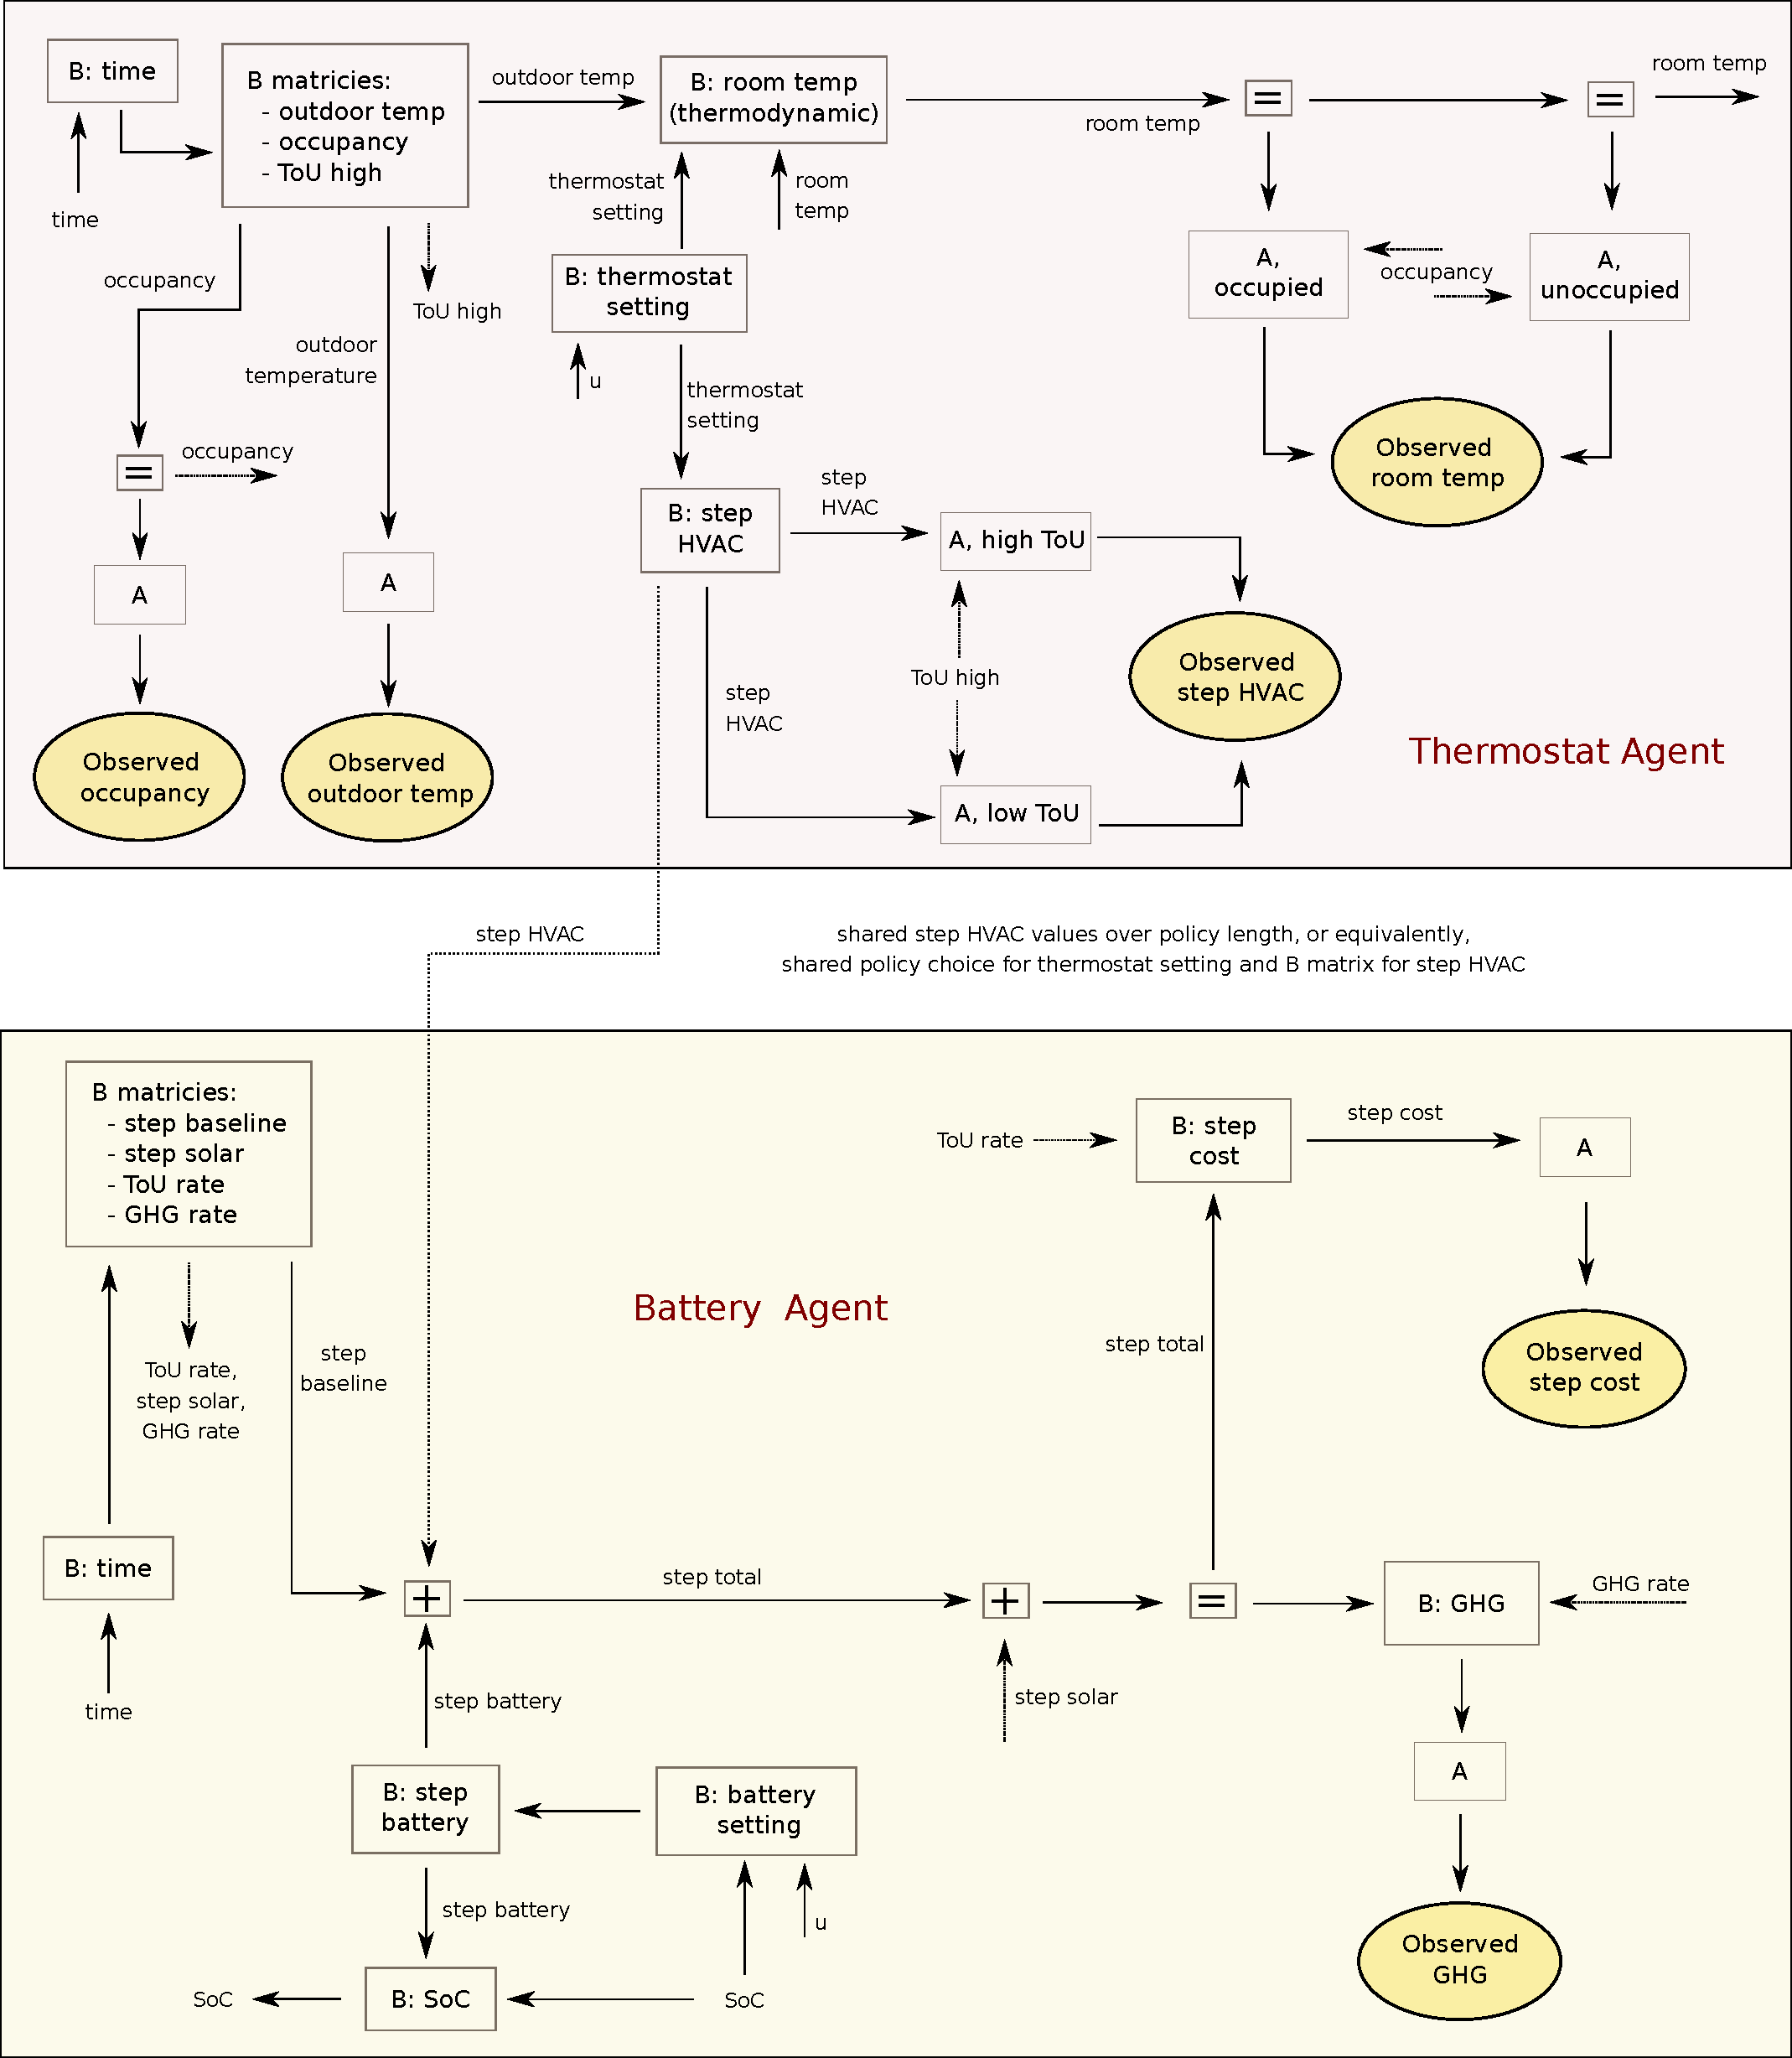
\includegraphics[width=0.85\columnwidth]{figures/multi_agent_plate_full}
\par\end{centering}
\caption{Pseudo-factor graph for two-agent EcoNet model. See text for meaning
of state and observation variables and for information shared between
agents. Squares labeled $A$ and $B$ refer to $A$ (likelihood) and
$B$ (prior transition) matrices in the pymdp implementation (see
Section~\ref{sec:model_description} for details on the $B$ matrix
structure). }\label{fig:factor=000020graph}
\end{figure}

\label{sec:model_description}
In the figure, variables \textit{step\_{*}} (e.g., \textit{step\_battery},
\textit{step\_solar}) refer to kWh energy use or generation associated
with a particular state variable. Total energy use in a simulation
step (\textit{step\_total}) is the sum of baseline, HVAC, battery,
and solar energy, where solar generation and battery discharge are
negative energies. The variable \textit{step\_cost} is the total cost
of energy in a simulation step (\textit{step\_total} $\times$ ToU
rate). Each of the yellow ellipses signify an observable, and each
is associated with a preference (which can be flat). \textit{SoC}
is battery state of charge. \textit{GHG} is greenhouse gas emissions.
\textit{ToU\_high} is a Boolean variable that signifies whether or
not the ToU rate is high or low.

The $B$ (transition) matrix for room temperature encodes a simple
thermodynamic model, where new room temperature depends on previous
room temperature, outdoor temperature, thermostat setting, and the
size of the HVAC system. The $B$ matrices for HVAC energy, battery
energy, SoC, and total energy also encode simple formulas (for example,
the formula for total energy was just given). Any degree of noise can
optionally be embedded in $A$ (likelihood) or $B$ matrices, in priors,
and/or in the underlying input data table. Parameter learning is also
possible.

\subsubsection{Predictive Transition Matrices for Exogenous Factors}
\label{sec:predictive_B}

In a standard POMDP formulation, the transition matrices for exogenous
state factors (outdoor temperature, occupancy, ToU period) are typically
set to identity matrices, encoding the assumption that these variables
do not change. This is a poor assumption for energy management, where
ToU rate transitions, occupancy changes, and temperature trends are
critical to planning ahead. An agent that assumes the current ToU period
will persist indefinitely cannot anticipate the value of pre-charging a
battery before a peak period begins.

We address this by constructing \emph{predictive $B$ matrices} that are
updated at each simulation step using available forecast information.
This approach is a natural application of the active inference framework:
the $B$ matrix encodes the agent's beliefs about state transitions, and
updating it with forecast data simply means providing the agent with
a more accurate generative model.

Three exogenous factors receive predictive updates:

\begin{itemize}
\item \textbf{$B_{\text{TOU}}$ (ToU period):} The time-of-use schedule is
published by the utility and is known in advance. At each step $t$, the
transition matrix is set deterministically: all columns map to the
ToU state at step $t+1$, i.e., $B_{\text{TOU}}[s_{t+1}, s_t, 0] = 1$
for the scheduled next-step value $s_{t+1}$.

\item \textbf{$B_{\text{occ}}$ (Occupancy):} The homeowner's occupancy
calendar is similarly known. The transition matrix is constructed
identically to $B_{\text{TOU}}$, deterministically encoding the
scheduled occupancy at the next step.

\item \textbf{$B_{\text{out}}$ (Outdoor temperature):} Short-term
weather forecasts provide a point estimate of the next-step outdoor
temperature. We encode this as a Gaussian kernel centered on the
forecast value (discretized to the nearest temperature bin) with
standard deviation $\sigma = 1$ bin, spanning $\pm 3$ bins:
\begin{equation}
B_{\text{out}}[j, i, 0] \propto \exp\left(-\frac{(j - \hat{j}_{t+1})^2}{2\sigma^2}\right)\,,
\label{eq:predictive_B_temp}
\end{equation}
where $\hat{j}_{t+1}$ is the discretized forecast temperature for
step $t+1$. Each column is normalized to sum to one.
\end{itemize}

The pymdp framework reuses the same $B$ matrix across all steps of a
policy rollout. This means the one-step prediction is accurate, while
multi-step rollouts approximate the true multi-step transition by
repeating the one-step forecast. This approximation is acceptable
because (i) the EFE naturally weights near-term predictions more
heavily, (ii) the same approximation is already used for the
controlled $B$ matrix (room temperature), and (iii) even one-step
accuracy represents a substantial improvement over the identity
assumption.

\subsubsection{Cost-Aware Thermostat Agent}
\label{sec:cost_aware}

The standard Thermostat Agent uses four state factors and has no
direct awareness of energy costs. To enable principled cost--comfort
trade-offs, we extend the generative model with a fifth state factor
(\emph{energy demand}, discretized into 10 levels from 0 to 9~kWh)
and a fifth observation modality (\emph{cost}, discretized into 5
levels). The cost observation enters through the standard $A$ matrix
likelihood: $A_{\text{cost}}$ maps joint states (energy demand $\times$
ToU period) to cost observations, encoding the agent's knowledge that
energy consumed during peak periods costs more than during off-peak.
A preference vector $C_{\text{cost}}$ encodes the household's
preference for low-cost outcomes, with amplitude scaled by a
\texttt{cost\_scale} parameter.

The transition matrix for the energy demand factor,
$B_{\text{energy}}$, is constructed using a \emph{phantom battery}:
a lightweight copy of the Battery Agent's generative model that is
rolled forward one step to predict $P(\text{charge}, \text{discharge},
\text{off})$. The resulting probability vector defines a mixture
transition matrix:
\begin{equation}
B_{\text{energy}}[j', j, a] = \sum_{b \in \{\text{ch}, \text{dis}, \text{off}\}} p(b)\,\delta_{j', \text{clip}(j + \Delta(a, b))}\,,
\label{eq:phantom_B}
\end{equation}
where $a$ is the HVAC action, $b$ indexes battery actions with
probability $p(b)$ from the phantom, and $\Delta(a, b)$ is the
discretized net energy change from HVAC action $a$ combined with
battery action $b$. The HVAC and energy demand actions are constrained
to be identical ($a_{\text{energy}} = a_{\text{HVAC}}$), reducing the
policy space from $3^{2T}$ to $3^T$.

This construction ensures that cost awareness enters through the
standard EFE computation (Equation~\ref{eq:EFE_decomp}): the risk
term drives the agent toward low-cost outcomes via $C_{\text{cost}}$,
while the ambiguity term captures uncertainty about energy demand
given the stochastic battery behavior. No ad hoc cost penalty or
modified objective is required.

\subsubsection{State Factor Summary}

The Thermostat Agent uses four state factors in its basic configuration:
room temperature (26 discrete levels), outdoor temperature (26 levels),
occupancy (2 levels: occupied or unoccupied), and ToU period (2 levels:
high or low). The cost-aware variant adds a fifth factor (energy demand,
10 levels). The Battery Agent uses three state factors: state of charge
(5 levels, from 0.0 to 1.0 in steps of 0.2), cumulative cost (10 levels),
and cumulative GHG emissions (10 levels). Each agent has 3 available
actions, and with a policy length of 6 steps, this yields $3^6 = 729$
candidate policies per agent per time step.

The Battery Agent employs a dynamic preference vector ($C$ vector) whose
values shift based on the current ToU period. During off-peak periods, the
agent prefers to charge (or hold), while during peak periods it prefers to
discharge. This is a principled use of active inference: the preferences
legitimately change with context, reflecting the household's conditional
goals. Formally, $p(o \mid C)$ in Equation~\ref{eq:EFE_decomp} is
conditioned on the current ToU observation, so the risk term automatically
drives the agent toward context-appropriate behavior without requiring
separate reward shaping.

The discretisation levels for cost, temperature, and energy are set
by the user. Choices affect the size of the $A$ and $B$ matrices.
A very high discretisation level would approximate a continuous state-space
model, but would incur a memory and run-time penalty. The most important
factor influencing run time is the policy length. We found that a
policy length of six steps (12 hours) is needed to allow the agent
to adequately plan ahead for battery charge and discharge in our sample
problems. A shorter policy length of four steps (8 hours) is used in
the coordination mode comparison experiments
(Section~\ref{sec:coordination_results}) to reduce computation time
for the multi-agent configurations; the deterministic and cost-aware
experiments use the full six-step horizon. Other hyperparameters include target room temperature for
occupied and unoccupied status, policy length, initial beliefs about
room temperature and SoC, the simulation length, and whether parameter
learning is used.

In each simulation step, the Thermostat Agent evaluates and selects
a best policy. It passes the impacts of that policy on HVAC energy
use to the Battery Agent. The Battery Agent considers HVAC energy,
along with other energies, when it estimates total energy and total
cost. This cascading update structure ensures that the Battery Agent's
planning accounts for the thermal load imposed by the Thermostat Agent's
decisions.

The model is constructed in pymdp \cite{Heins_2022}. State transitions
are updated sequentially, such that the update of one state variable
can be used as input for updating other state variables. For example,
solar generation is updated based on lookup to the input data table.
The result of this update is used as input for updating total energy
(\textit{step\_total}). We used a modified version of pymdp that allows
this kind of cascading updates.

Figure \ref{fig:outdoor_temp} shows an example of input data, in
this case outdoor temperature and baseline energy use.

\begin{figure}
\begin{centering}
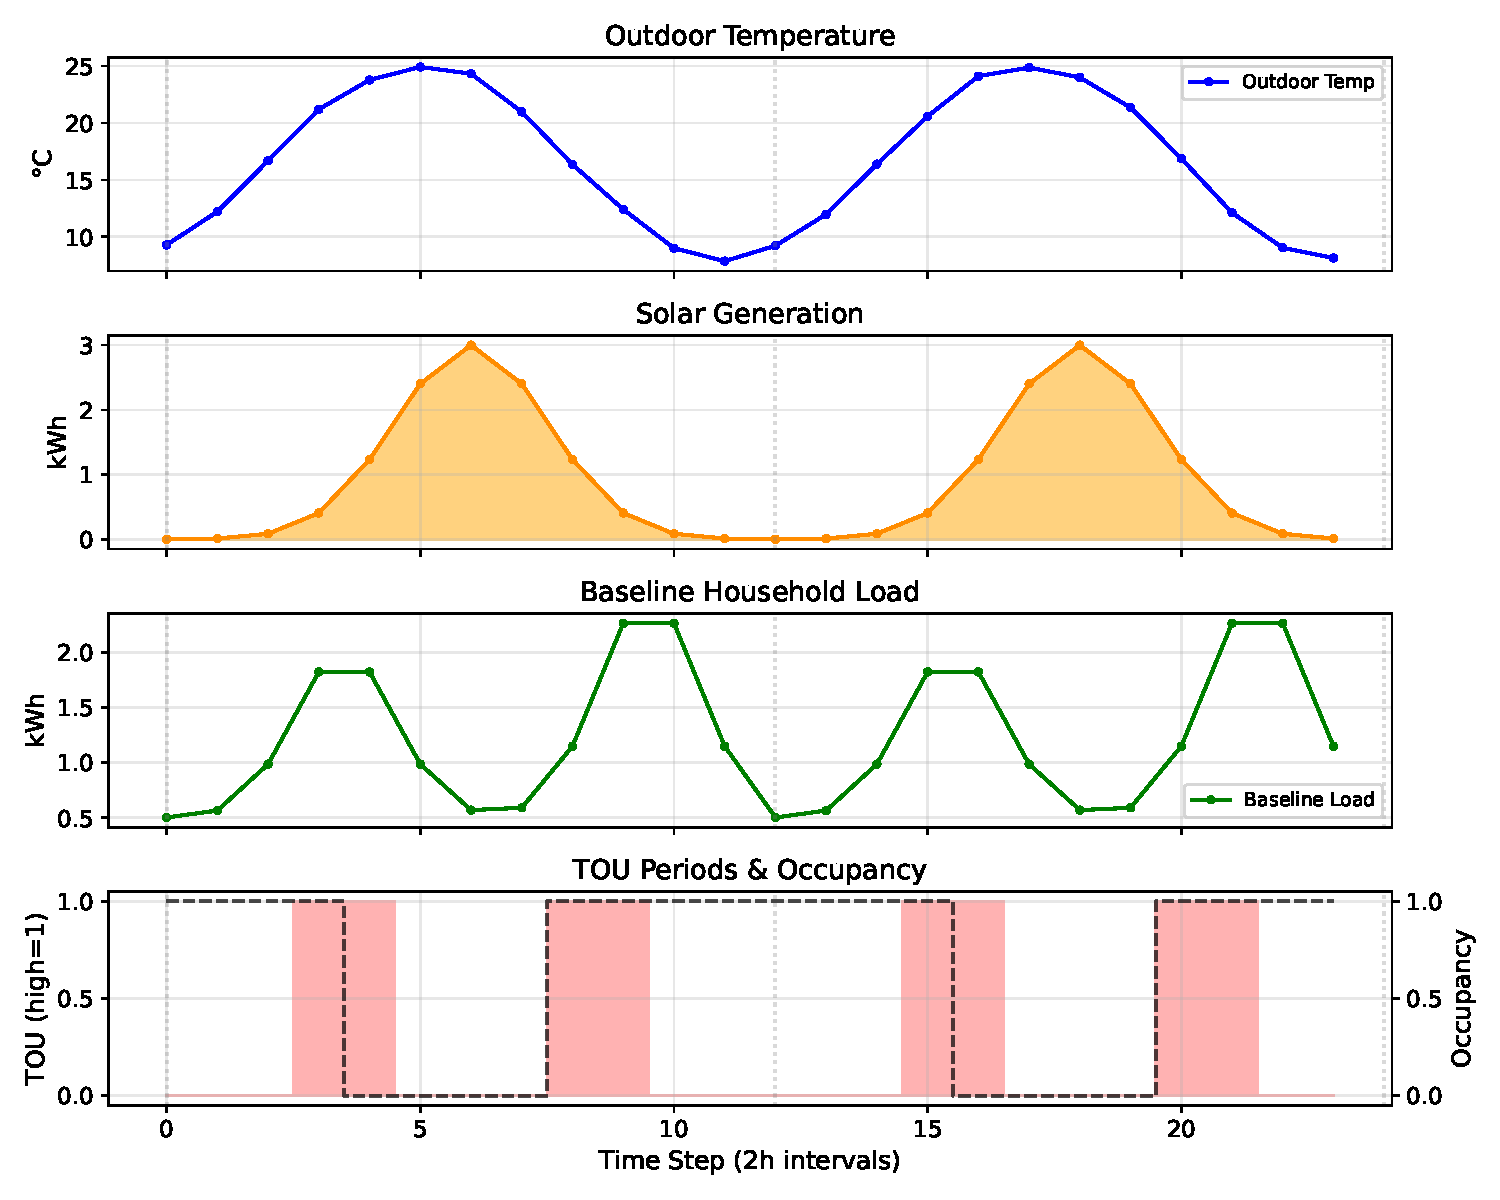
\includegraphics[width=0.85\columnwidth]{figures/input_temperature}
\par\end{centering}
\caption{Daily outdoor temperature and baseline energy use as examples of input
data (top and bottom panels). Shading indicates occupancy status.
Target temperatures for occupied and unoccupied status are prior preferences
set by the user. The middle panel shows cumulative absolute difference
between outdoor temperature and targets. This is the worst case scenario
for indoor room temperature, for a house without a HVAC system. }\label{fig:outdoor_temp}
\end{figure}


\subsection{Coordination Modes}\label{sec:coordination}

A key question in multi-agent HEMS is how agents should coordinate their
actions. We investigate five coordination modes of increasing sophistication:

\textbf{Independent.} Each agent uses static preference vectors ($C$ vectors)
that do not adapt to context. The Thermostat Agent always prefers target
temperature; the Battery Agent always prefers low cost. There is no
inter-agent coordination signal beyond the cascading update structure
described above.

\textbf{Aligned (decentralized).} Each agent dynamically adjusts its
$C$ vector based on shared environmental signals (ToU period, occupancy).
During peak periods, the Battery Agent's preference for discharge increases;
the Thermostat Agent relaxes comfort preferences when unoccupied. Agents
independently respond to the same context without explicit communication.

\textbf{Hierarchical (centralized).} A meta-agent observes both agents'
states and explicitly sets their $C$ vectors to achieve global coordination.
This centralizes decision-making but requires full observability of both
agents' hidden states.

\textbf{ToM + Belief Sharing (decentralized).} Following Friston et al.
\cite{friston2024federated}, agents share posterior beliefs rather than
raw states, enabling decentralized consensus formation. This mode extends
the Aligned mode with three additions: a belief sharing channel, an
auditory likelihood mapping, and a Theory of Mind meta-inference layer.

In the \textit{belief sharing channel}, the Thermostat Agent projects its
room temperature posterior $q(\text{room\_temp}) \in \mathbb{R}^{26}$ to a
5-level comfort belief $q(\text{comfort}) \in \{\text{COLD}, \text{COOL},
\text{COMFY}, \text{WARM}, \text{HOT}\}$ and shares it with the Battery
Agent. The Battery Agent shares its native $q(\text{SoC}) \in \mathbb{R}^5$
with the Thermostat Agent. Crucially, agents share full probability
distributions, preserving uncertainty information
\cite{vasil2020world}.

The \textit{auditory A matrix}\footnote{The term ``auditory'' follows the
neuroscience convention where agents receive social information through a
sensory channel analogous to hearing. In the HEMS context, this corresponds
to a communication channel (e.g., a local network message) through which one
agent receives the other's belief report.} extends each agent's generative model with
an additional observation modality for received beliefs. A likelihood
mapping $A_{\text{aud}}$ encodes prior expectations about the other
agent's state. The Thermostat Agent models
$P(o_{\text{soc}} \mid \text{room\_temp})$, its expectation of battery
SoC given its own thermal state, while the Battery Agent models
$P(o_{\text{comfort}} \mid \text{SoC})$. This ``auditory'' mapping
follows the communication-as-observation principle from federated inference
\cite{friston2024federated,friston2020linguistic}, and ensures that social preferences emerge
naturally within pymdp's standard EFE computation:
\begin{equation}
G(\pi) = \sum_{m \in \text{self}} \left[\text{risk}_m + \text{ambiguity}_m\right]
       + \underset{G_{\text{social}}}{\underbrace{\text{risk}_{\text{aud}} + \text{ambiguity}_{\text{aud}}}}\,.
\label{eq:social_efe}
\end{equation}

Finally, the \textit{Theory of Mind} layer provides meta-inference: each
agent maintains a Bayesian filter that tracks the other agent's hidden
state over time, using received beliefs as observations. A reliability
parameter $\rho$ tracks the consistency between received and predicted
beliefs via exponential moving average:
\begin{equation}
\rho_t = (1 - \alpha)\,\rho_{t-1} + \alpha\,(1 - \|\mathbf{q}_{\text{received}} - \mathbf{q}_{\text{predicted}}\|)\,,
\label{eq:reliability}
\end{equation}
where $\alpha = 0.1$ is the learning rate. This reliability gates the
effective social preference weight, ensuring that agents fall back to
self-interest when the other's reports are unreliable.

The belief-sharing architecture is depicted in Figure~\ref{fig:belief_sharing}.
Messages are passed in a cascade: at each time step, the Thermostat Agent
first receives the Battery Agent's $q(\text{SoC})$ from the previous step,
infers and acts, then shares its $q(\text{comfort})$. The Battery Agent
receives this same-step comfort belief, infers and acts, and stores its
$q(\text{SoC})$ for the next step. The one-step delay for the
battery-to-thermostat channel creates anticipatory dynamics, requiring the
Thermostat Agent's ToM filter to predict the Battery Agent's future state.

\textbf{Sophisticated (mutual phantom inference).} Each agent maintains
a lightweight copy---a \emph{phantom}---of the other agent's generative
model. The Thermostat Agent uses a phantom Battery Agent to predict the
probability of battery charge, discharge, or idle actions over the planning
horizon. These predictions are used to construct the energy demand
transition matrix $B_{\text{energy}}$ (Equation~\ref{eq:phantom_B}),
enabling the Thermostat Agent to anticipate cost consequences of its HVAC
decisions. Conversely, the Battery Agent uses a phantom Thermostat Agent
to predict future HVAC activity, constructing step-dependent energy
transition matrices for its own EFE computation. Both agents also use
predictive $B$ matrices for exogenous factors
(Section~\ref{sec:predictive_B}), enabling them to anticipate ToU
transitions and temperature trends. This mode represents a form of
implicit Theory of Mind: each agent models the other's decision process
without direct communication, relying instead on shared knowledge of
the environment and the other's generative model structure
\cite{pitliya2025theory}.

\begin{figure}[htbp]
\centering
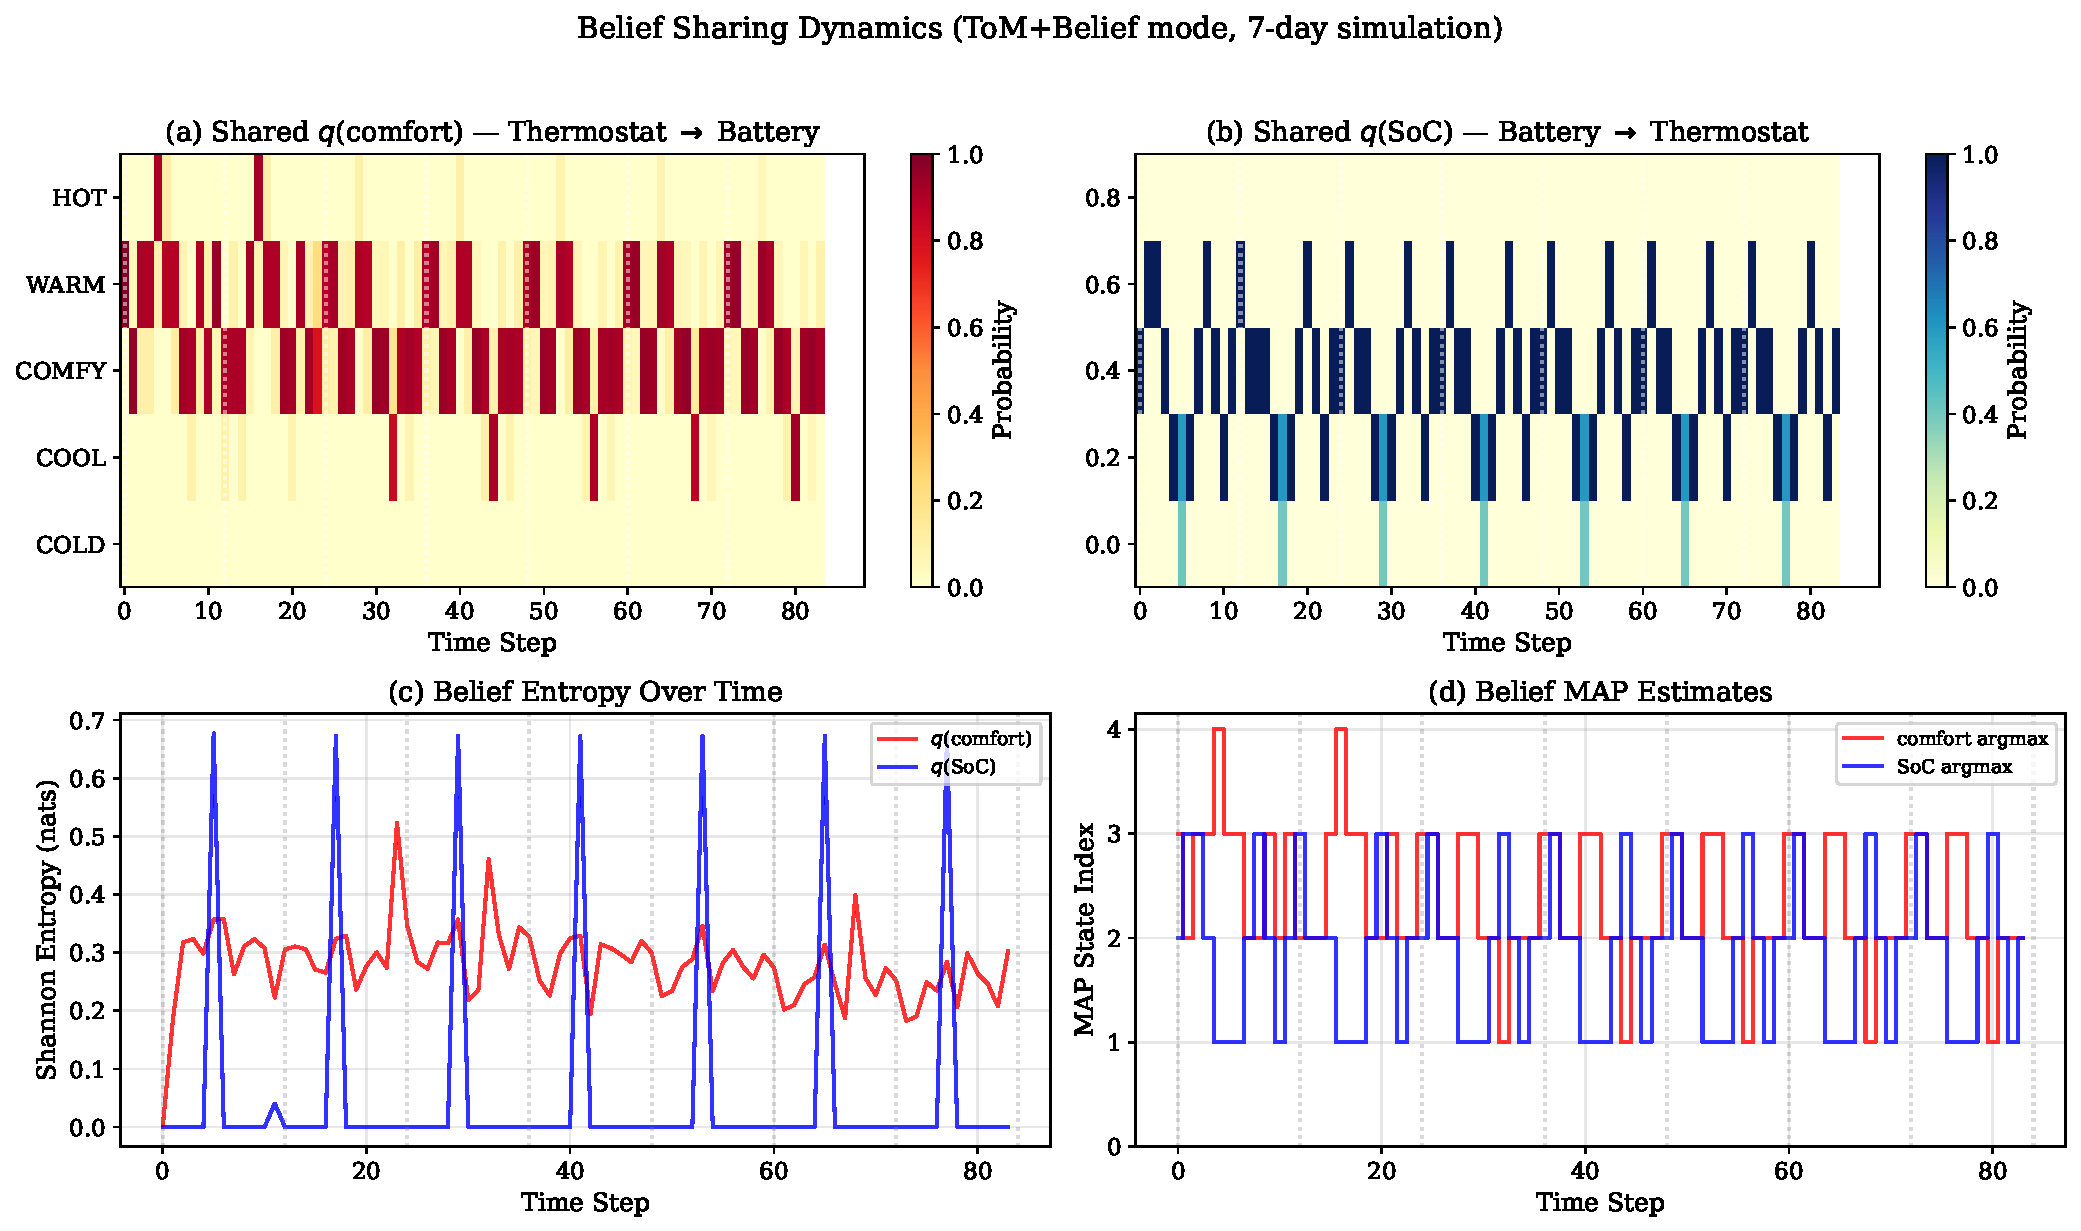
\includegraphics[width=0.85\columnwidth]{figures/fig16_belief_dynamics}
\caption{Belief sharing dynamics over a 7-day simulation in ToM+Belief mode.
(a)~Shared comfort posterior $q(\text{comfort})$ from the Thermostat Agent.
(b)~Shared SoC posterior $q(\text{SoC})$ from the Battery Agent.
(c)~Shannon entropy of shared beliefs over time.
(d)~MAP estimates of shared beliefs.}\label{fig:belief_sharing}
\end{figure}


\section{Results}

The experimental setup allows for flexible changes to parameters,
hyperparameters, priors, and input data. This permits us to run simulations
under a variety of conditions, of different degrees of challenge.
Unless otherwise noted, all experiments use precision parameter
$\gamma = 16$ and 2-hour time steps. The deterministic and baseline
comparison experiments use 2-day synthetic data with a policy length
of 6 steps (12 hours). The multi-seed coordination and Oracle gap
experiments (Sections~\ref{sec:coordination_results}
and~\ref{sec:cost_aware_results}) use 7-day synthetic data, a policy
length of 4 steps (8 hours), predictive $B$ matrices, and $B$-learning
disabled (i.e., transition dynamics are specified, not learned online).
Results are averaged over 5 random seeds
$\{42, 137, 256, 789, 1024\}$. The cost-aware
(Sophisticated) mode uses a policy length of 6 steps where noted.
In this section, we present results for seven experimental analyses:
(1) a deterministic problem with accurate agent models;
(2) a parameter learning scenario where the thermodynamic model is unknown;
(3) a baseline comparison against unmanaged and rule-based controllers;
(4) a climate sensitivity analysis using real weather data from four cities;
(5) a validation analysis confirming physical constraint adherence;
(6) a coordination mode comparison including Theory of Mind with belief sharing; and
(7) a cost-aware planning analysis with predictive transition matrices
and sophisticated mutual inference.

\subsection{Deterministic Scenario}

The first scenario is a deterministic problem (zero uncertainty) where the
agents have accurate models of the environment. The policy length
is six steps (12 hours), and we also show results for a modified problem
that has four steps. Two days are simulated. The input data are the
same for each day. ToU rates are either high or low, and these are
associated with numerical values.

The results demonstrate that the agents try to achieve and maintain
target room temperatures, in spite of the under-powered HVAC system.
They also try to reduce costs and plan ahead to charge the battery
for later use.

Figure \ref{fig:B-neg_efe} shows the distribution of (negative) expected
free energy (i.e., $G_{\pi}$ from Equation~\ref{eq:EFE}) over all policies for the Battery Agent
(each agent evaluated 729 policies in each simulation step). Negative
EFE for the selected policy in each simulation step is shown in red,
which by design coincides with the maximum $G_{\pi}$ (policy selection
was deterministic). In each step, the agent takes the first action
in the selected policy. As shown, the EFE landscape varies across
simulation steps---the policies at each time step result in a range
of EFE values. Because EFE is the sum of information gain and expected
utility, a change in either across simulation steps can result in
policies that the agent has more or less commitment toward. By construction,
the average EFE corresponds to the entropy or uncertainty of (Bayesian)
beliefs about the policies that should be pursued. Fluctuations in
this uncertainty reflect the challenge of satisfying multiple constraints
or preferences in a context-sensitive fashion.

\begin{figure}
\begin{centering}
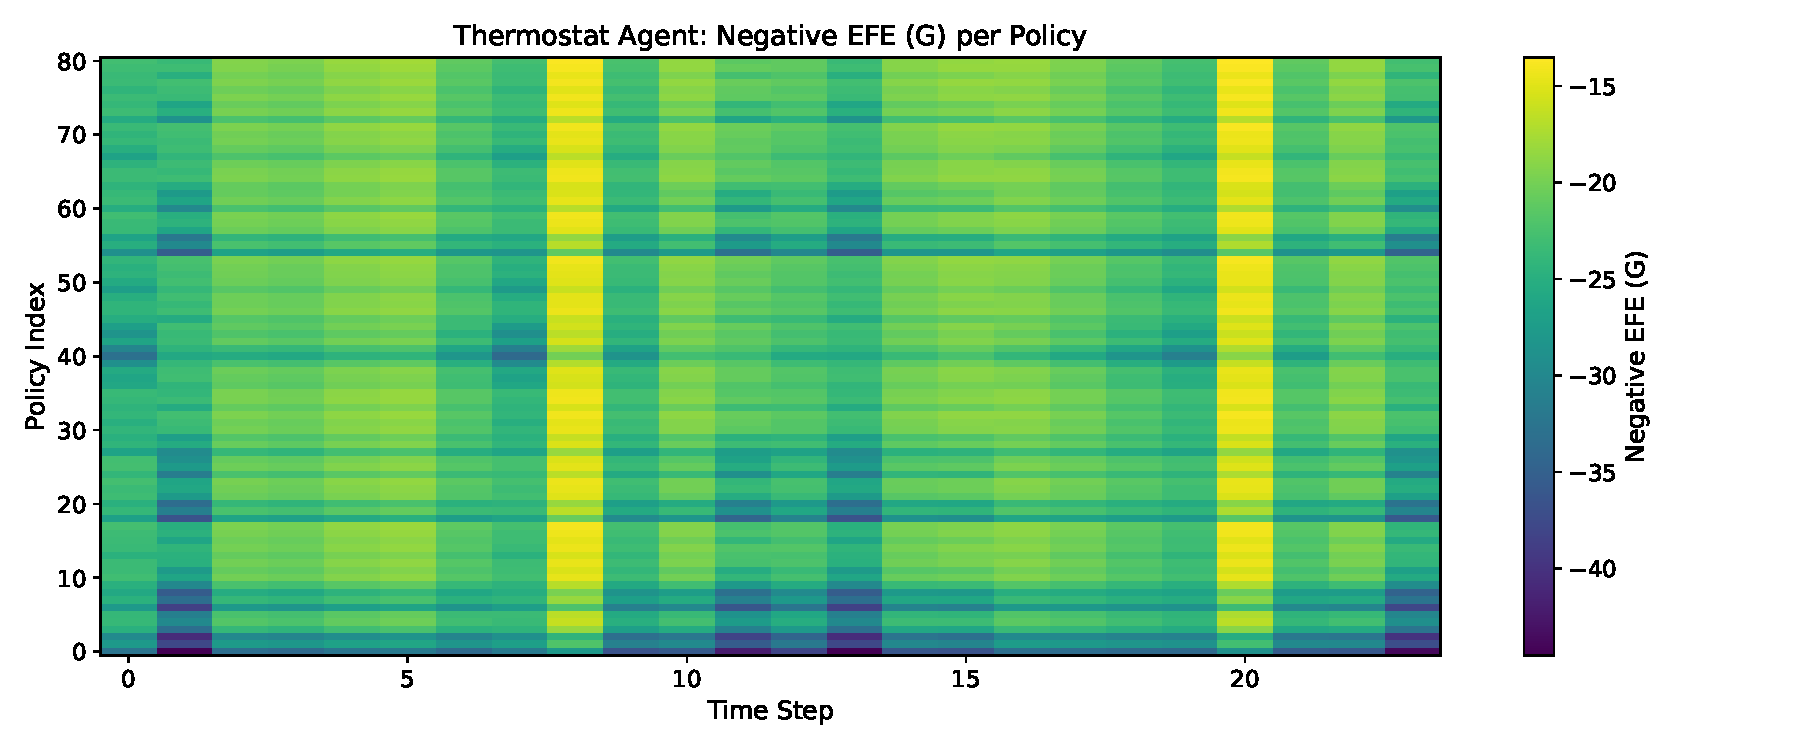
\includegraphics[width=0.7\columnwidth]{figures/A_efe}
\par\end{centering}
\caption{Distribution of negative EFE over policies and simulation steps. }\label{fig:B-neg_efe}
\end{figure}

Figure \ref{fig:A-temperature}, top panel, shows observed outdoor
and room temperatures, given the series of actions selected by the
agents. In a worst case scenario, for a house with no HVAC system,
the two curves would be superimposed. The middle panel shows the difference
between observed room temperature and target temperatures ($18^{\circ}$C
for occupied status, $16^{\circ}$C for unoccupied). The daily average
cumulative sum of absolute temperature differences from the targets
is 22 degrees C, which is less than the worst case of 64 degrees,
shown in Figure \ref{fig:outdoor_temp}. The bottom panel shows the
selected thermostat actions.

The Thermostat Agent tends to turn on the heat when the room is below
the target temperatures and turn on the air conditioning (ac) when
the room is above the target temperatures. Its actions cannot maintain
target room temperatures, however, because the HVAC system is underpowered.
We designed the HVAC system this way to challenge the agent. As would
be expected, the largest differences between targets and room temperature
occur during cool nights and warm afternoons.

\begin{figure}
\begin{centering}
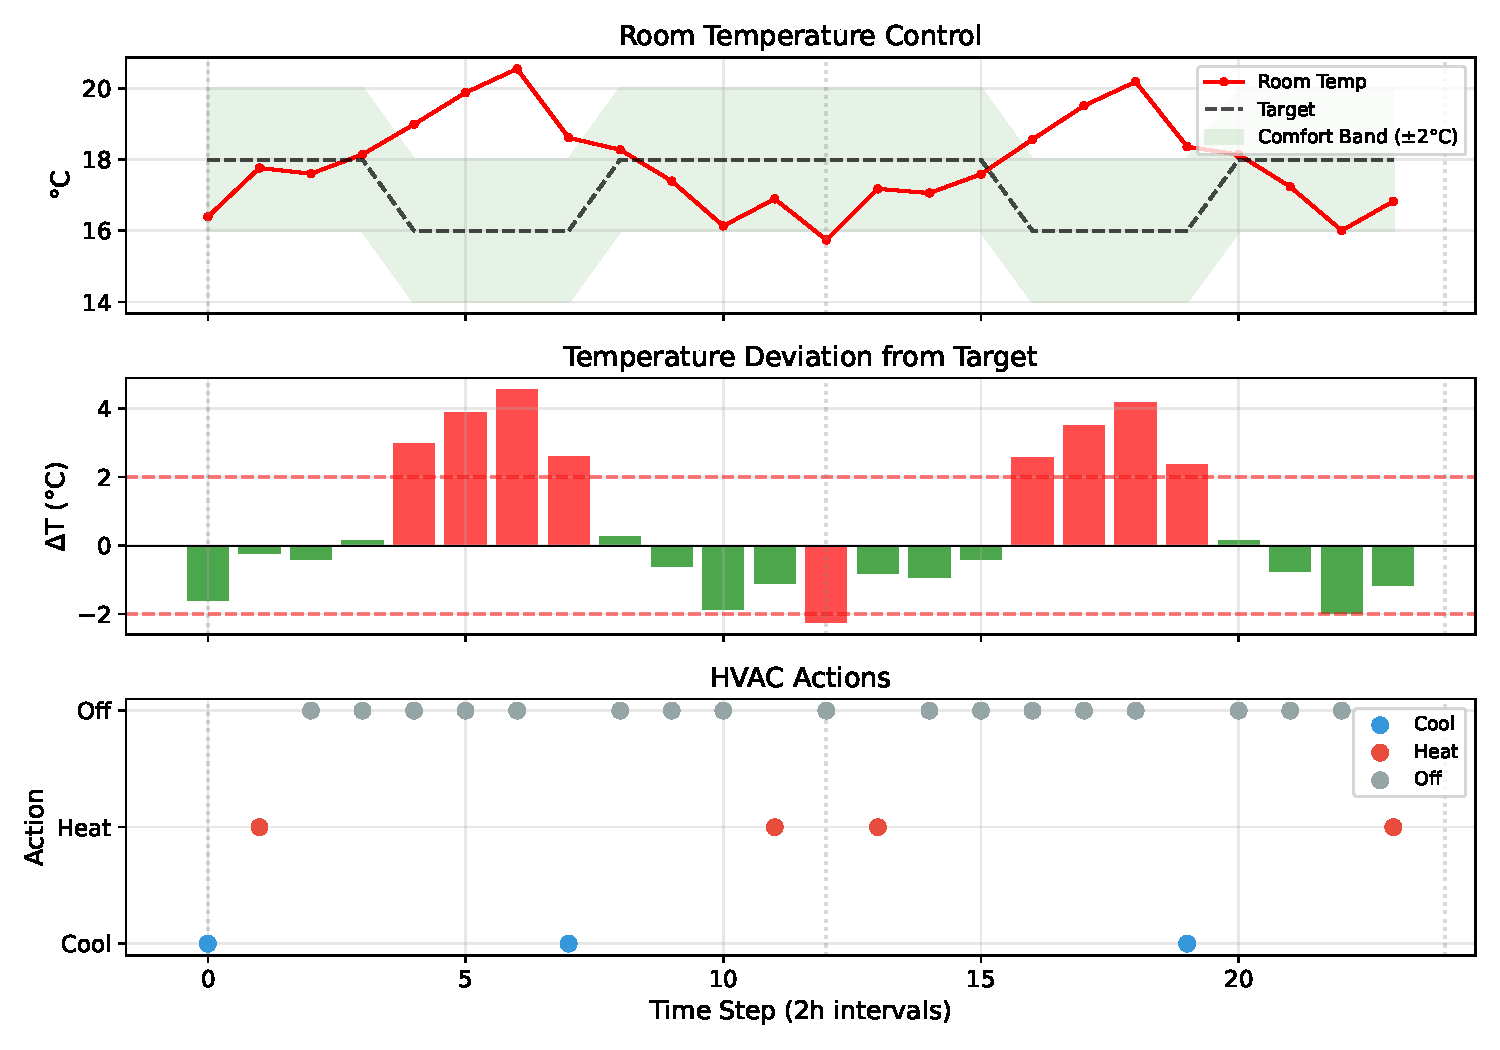
\includegraphics[width=0.85\columnwidth]{figures/A_temperature}
\par\end{centering}
\caption{Observed outdoor and room temperatures (top panel). Difference between
observed room temperature and targets (middle panel). The selected
thermostat actions (bottom panel). }\label{fig:A-temperature}
\end{figure}

The Battery agent has a preference to minimize energy costs. One way
it can do so is to discharge the battery during high-ToU periods,
when energy is expensive. Discharged energy is used by the household,
if needed, and any excess is sold back to the grid. Figure \ref{fig:B-soc-vs-tou}
shows that the agent tends to use the battery (indicated by a drop
in SoC) during high-ToU periods (red shading). Similarly, it tries
to charge the battery during low-ToU periods.

Battery SoC is discretized into five categories, from 0.0 to 1.0 in
steps of 0.2. The battery has a one-way efficiency of $\eta = 0.9$
(round-trip efficiency 81\%), meaning that charging draws
$\Delta\text{SoC} \times C / \eta$ from the grid while discharging
delivers $\Delta\text{SoC} \times C \times \eta$ to the household,
where $C = 5$~kWh is the total capacity.
To protect the battery, the Battery Agent is not allowed
to discharge when SoC $\leq$ 0.2 or to charge when SoC $\geq$ 0.8.
Each two-hour step can charge or discharge the battery 20 percent.
The initial charge is 0.2. Starting from an SoC of 0.2, the agent
can maximally charge the battery in three consecutive two-hour blocks.
It never needs to charge the battery to a SoC of 0.8, however, because
all high ToU periods last for no more than two steps. The charges
it attains are sufficient to cover all high-ToU periods.

\begin{figure}
\begin{centering}
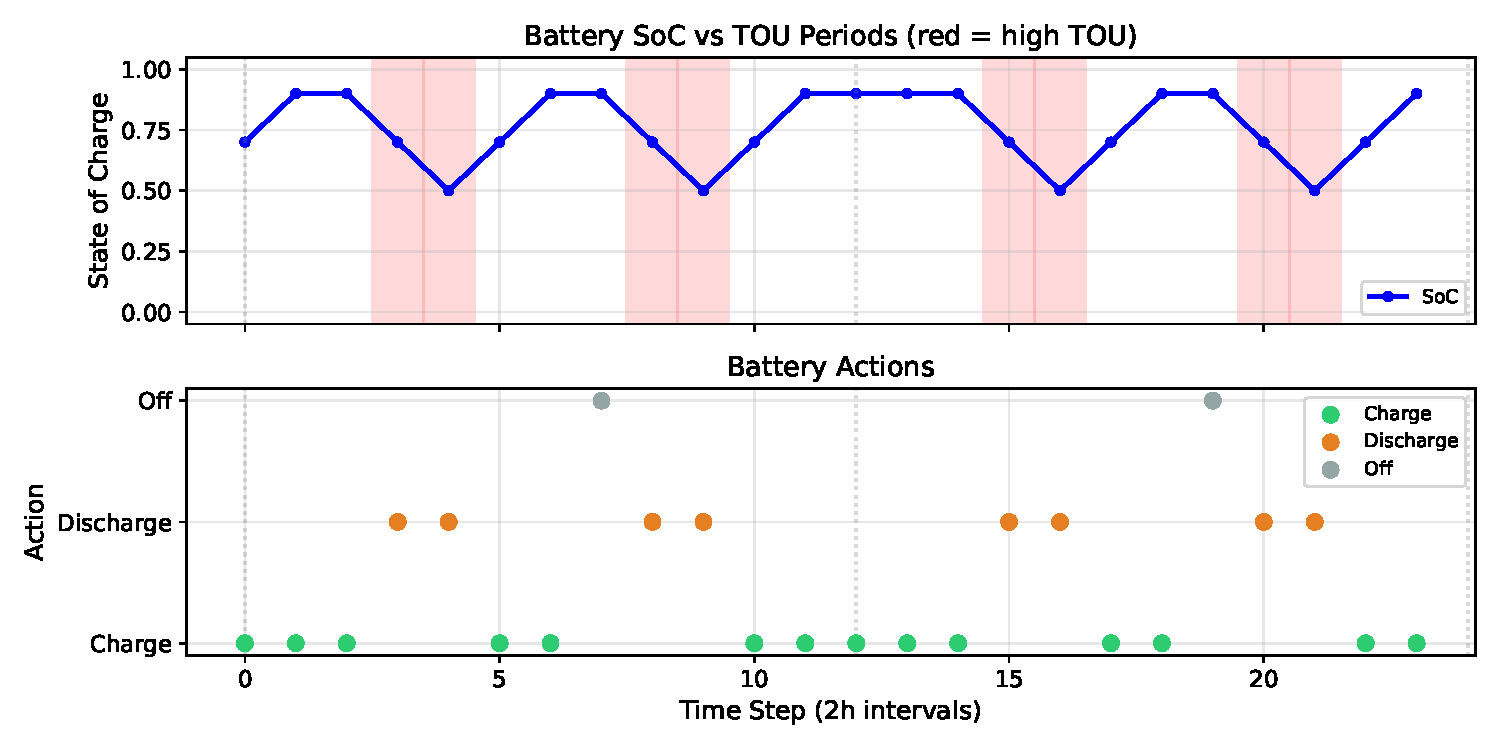
\includegraphics[width=0.7\columnwidth]{figures/B_battery}
\par\end{centering}
\caption{Agent beliefs about battery state of charge. Beliefs about ToU rates
are shaded. }\label{fig:B-soc-vs-tou}
\end{figure}

As a variation of this problem, we alter the ToU schedule so that
during each evening there is a three-hour high-ToU period. The policy
length is again six steps. Now the agent charges the battery fully
(to a SoC of 0.8) so that it can discharge during all high-ToU steps.
Results are shown in Figure \ref{fig:variation} (left panel). As
another variation, we run the same simulation but this time using
a policy length of four steps (eight hours). Now the agent cannot
see far enough into the future to perfectly plan ahead for the three-hour
high-ToU period. It starts charging too late, and as a result cannot
discharge during all high-ToU steps.

\begin{figure}
\begin{centering}
\begin{tabular}{|c|c|}
\hline
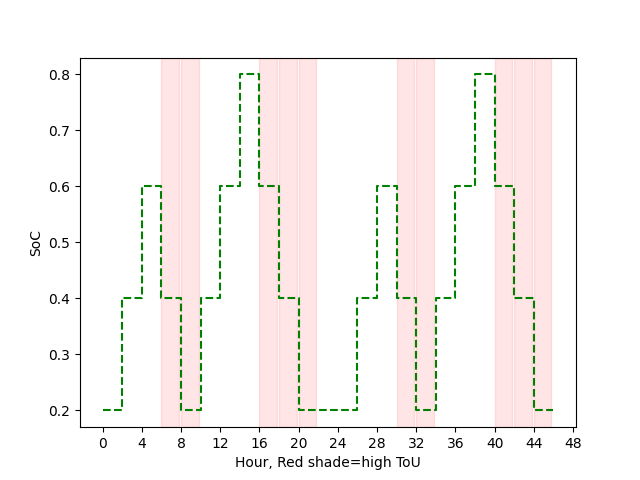
\includegraphics[width=0.45\columnwidth]{figures/B_battery_version2}  & 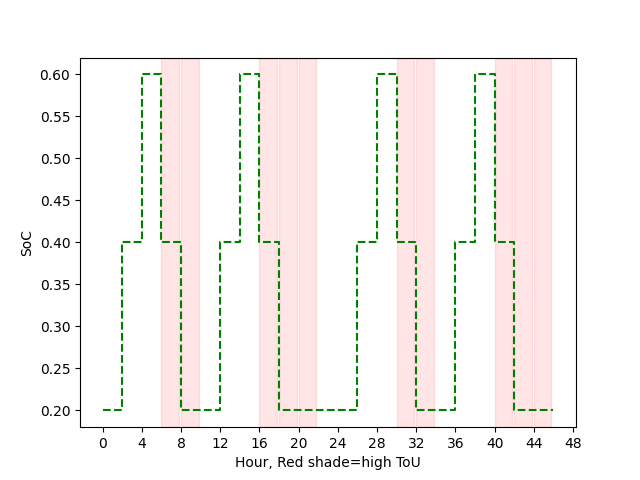
\includegraphics[width=0.45\columnwidth]{figures/B_battery_version3}\tabularnewline
\hline
\end{tabular}
\par\end{centering}
\caption{Agent beliefs about battery state of charge when an evening high-ToU
period last for three hours. Policy length is six steps (left panel)
and four steps (right panel). Beliefs about ToU rates are shaded.
}\label{fig:variation}
\end{figure}

Figure \ref{fig:B-step-cost-vs-tou} shows total energy use in the
house during each step of the original problem, along with solar generation
and battery charge and discharge. HVAC and baseline energy are not
shown. Battery charge registers as a positive energy, and discharge
and solar generation as negative energy. The four largest positive
peaks in total energy roughly coincide with morning and evening peak
baseline energy use, but are offset by the agent to occur during low-ToU
periods. The two largest negative peaks roughly coincide with solar
generation, but are offset to occur during high-ToU periods. The battery
only charges during low-ToU periods and only discharges during high-ToU
periods. Charging also tends to coincide with solar generation.

\begin{figure}
\begin{centering}
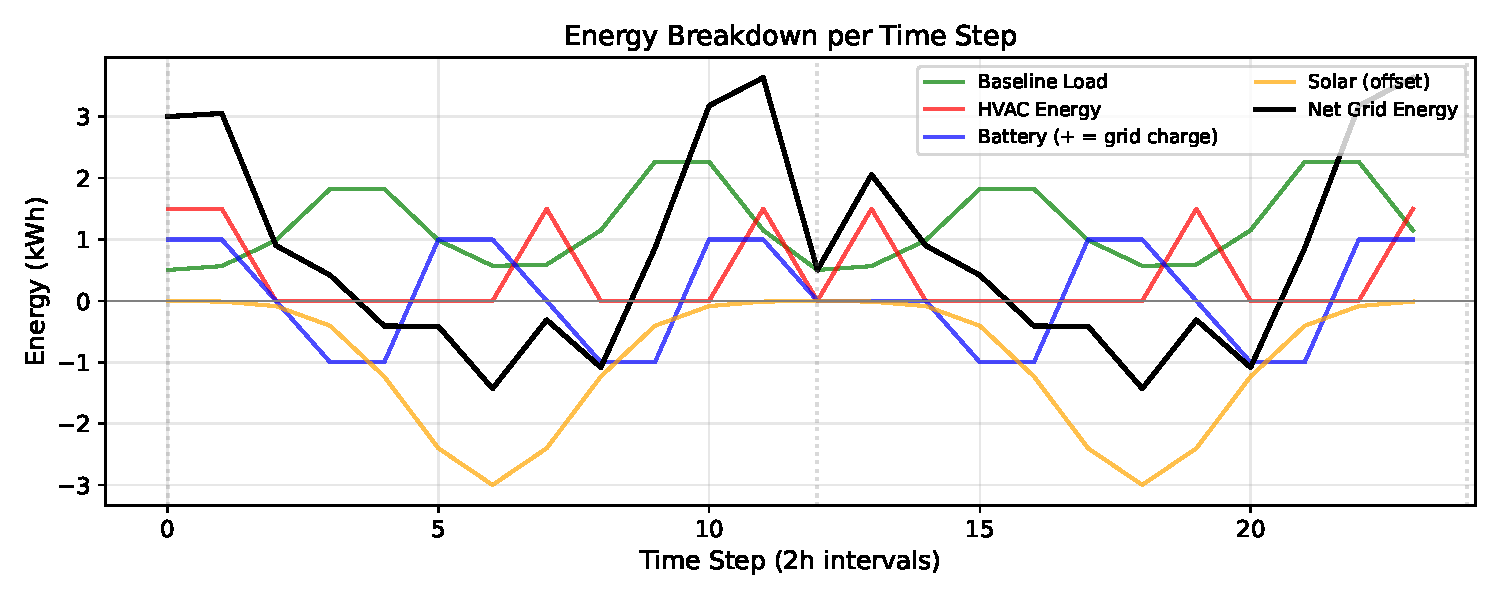
\includegraphics[width=0.7\columnwidth]{figures/B_energy_use}
\par\end{centering}
\caption{Agent beliefs about total, battery, and solar energy use. }\label{fig:B-step-cost-vs-tou}
\end{figure}

Figure \ref{fig:B-ghg} shows agent beliefs about total energy use
in comparison to grid-associated GHG rates (top panel). Peak energy
use is offset by the agent to avoid high-GHG rate periods. The bottom
panel shows beliefs about GHG emissions due to energy use.

\begin{figure}
\begin{centering}
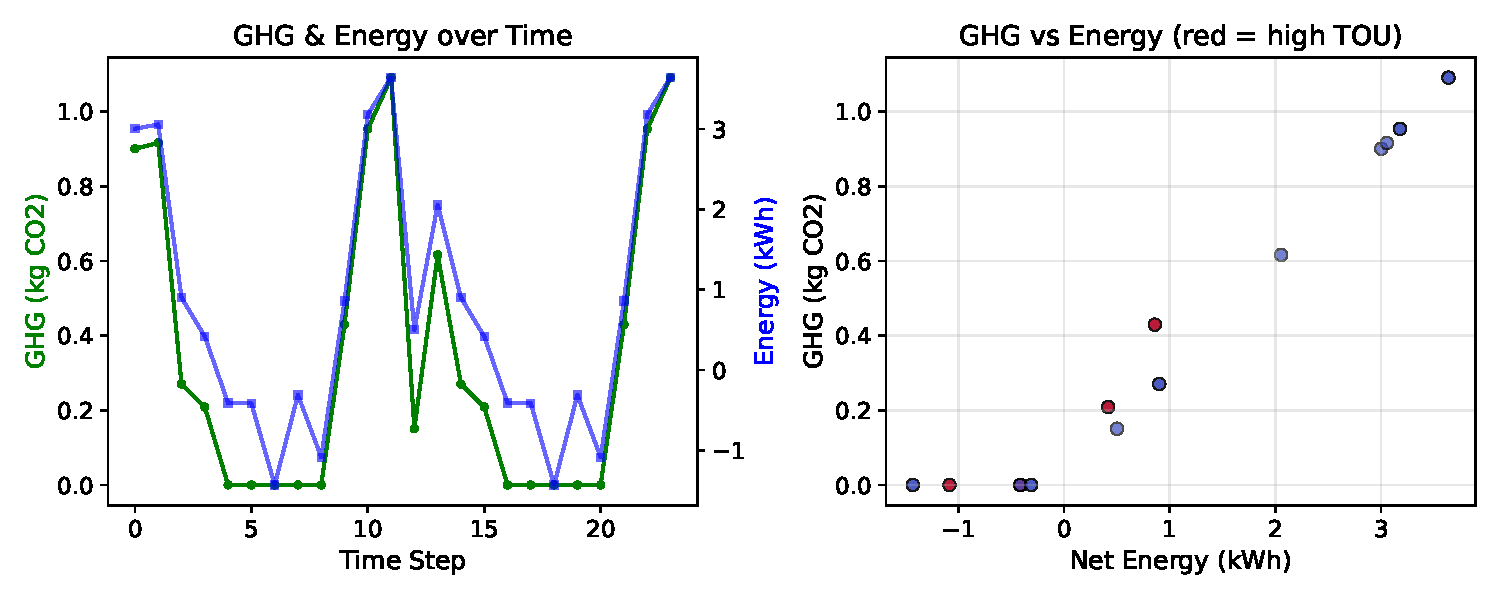
\includegraphics[width=0.85\columnwidth]{figures/B_GHG_emissions}
\par\end{centering}
\caption{Agent beliefs about total energy use versus grid-associated GHG rates
(top panel) and emissions due to energy use (bottom panel). Deeper
red shading indicates higher GHG rates. }\label{fig:B-ghg}
\end{figure}


\subsection{Parameter Learning Scenario}

The second scenario investigated is identical to the deterministic
case, but now the Thermostat Agent starts with an uninformative transition
matrix for room temperature, and an uninformative belief about initial
room temperature. In effect, the agent needs to learn the thermodynamic
model of the house. The $B$ matrix for room temperature is learned
via Dirichlet concentration parameter updates: after each observed
transition, the corresponding concentration parameter is incremented,
so that the agent's model gradually converges to the true transition
probabilities.

Figure \ref{fig:learning} shows the results of a 10-day learning run.
The top panel shows that the mean absolute EFE drops during learning,
as the agent becomes more confident about inferred policies. The bottom
panel shows that the daily cumulative temperature deviation decreases
as the learned transition model converges to the true dynamics. EFE
convergence was observed within approximately 5 days, and the system
achieved an average daily cost of \$1.27 and total GHG emissions of
32.86 kg CO$_2$ over the 10-day period. In a realistic setting, some
information about the thermodynamic model would likely be available,
and if so the transition matrix might need to be refined, rather than
learned from scratch.

\begin{figure}
\begin{centering}
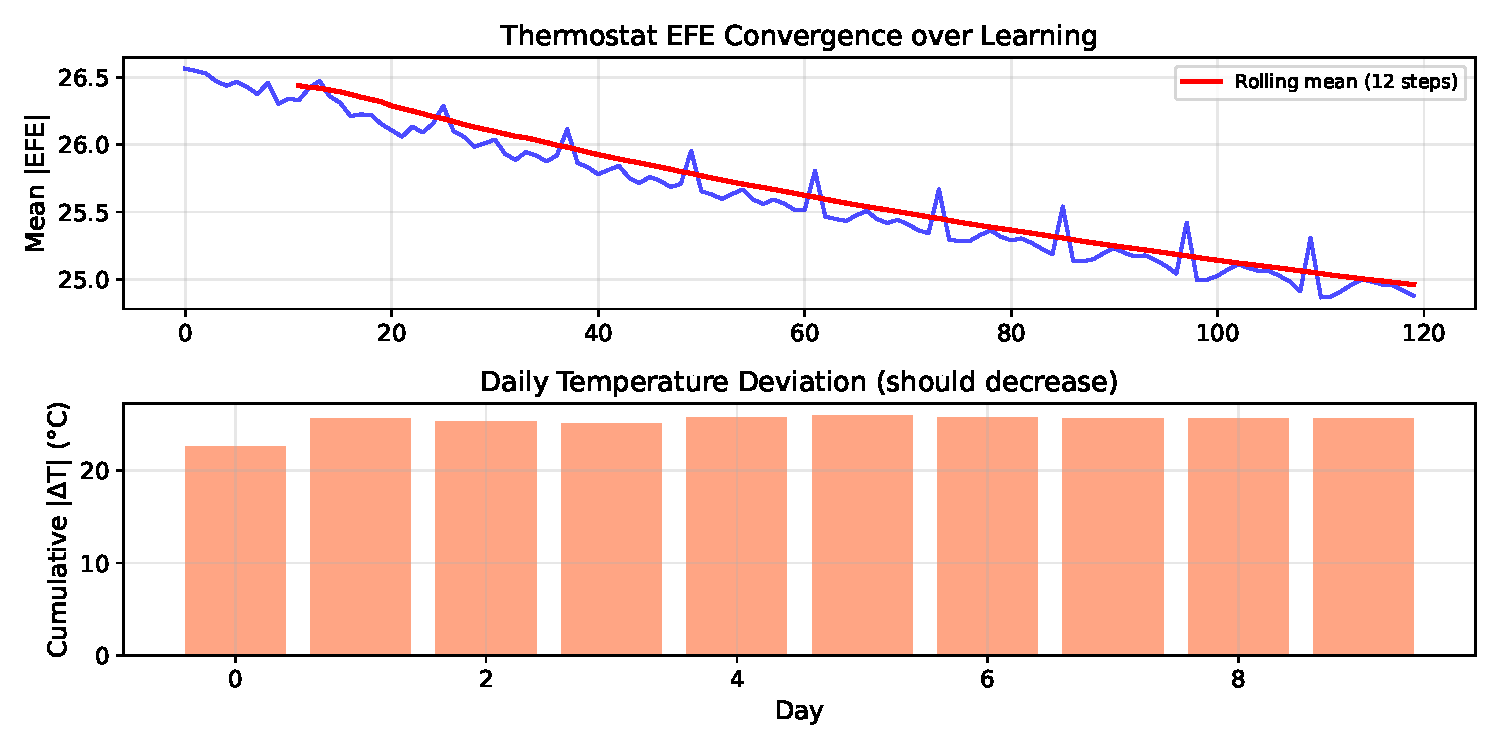
\includegraphics[width=0.85\columnwidth]{figures/learning_convergence}
\par\end{centering}
\caption{Learning the room temperature transition matrix over a 10-day period.
Top panel: EFE convergence showing the agent becomes increasingly confident
about inferred policies. Bottom panel: daily cumulative temperature deviation
decreases as the agent learns the thermodynamic model.}\label{fig:learning}
\end{figure}


\subsection{Baseline Comparison}\label{sec:baseline}

To quantify the benefit of active inference control, we compare EcoNet
against four baselines over a 2-day simulation period:

\begin{itemize}
\item \textbf{No-HEMS}: The household has a basic programmable thermostat
with a $\pm 1^{\circ}$C deadband around the target temperature (occupancy-aware),
but no battery management. This represents a typical home without an
energy management system.
\item \textbf{Rule-Based}: A simple rule-based controller that
charges the battery when solar generation exceeds load during off-peak periods,
discharges during high-ToU periods, and sets the
thermostat based on a fixed temperature threshold with occupancy awareness.
\item \textbf{MPC}: Model Predictive Control with a rolling 6-step (12-hour)
planning horizon, using backward induction DP at each step with perfect
knowledge of the system model.
\item \textbf{RL}: Tabular Q-learning with a coarse state space (200 states),
trained for 500 episodes on the same environment, then evaluated greedily.
\end{itemize}

Table \ref{tab:baseline} summarizes the 2-day results.\footnote{The
2-day baseline comparison uses the initial experimental configuration
(policy length 6, single seed). The comprehensive multi-seed evaluation
is presented in Tables~\ref{tab:coordination} and~\ref{tab:oracle_gap}.}
EcoNet achieves the lowest total cost (\$3.17) and lowest GHG emissions
(7.25 kg CO$_2$). The rule-based controller performs worst because it
does not plan ahead: it cannot anticipate high-ToU periods to pre-charge
the battery. The No-HEMS baseline avoids the worst excesses of the
rule-based controller (since the battery is simply off), but misses the
cost savings available from strategic charge/discharge scheduling.
EcoNet's battery utilization of 79.2\% with 1.70 full equivalent cycles
over the 2-day period indicates effective use of available storage
capacity.

The MPC and RL baselines provide important context for interpreting
EcoNet's performance. MPC with a 4-step horizon (matching the AIF
agents' policy length) achieves near-Oracle performance, as expected
for a method with perfect model knowledge over the planning horizon.
However, MPC requires an explicit, accurate model of system dynamics
and does not naturally handle model uncertainty or online learning.
The tabular Q-learning baseline, while achieving reasonable performance
after 500 training episodes, requires offline training on the
specific environment and lacks built-in uncertainty quantification.
EcoNet's active inference agents operate without offline training,
naturally quantify uncertainty through posterior beliefs, and can learn
unknown parameters online---advantages that become increasingly important
as the environment becomes less predictable.

\begin{table}[htbp]
\centering
\caption{Baseline comparison over a 2-day simulation period.}\label{tab:baseline}
\begin{tabular}{lccc}
\toprule
\textbf{Metric} & \textbf{EcoNet} & \textbf{No-HEMS} & \textbf{Rule-Based} \\
\midrule
Total cost (\$) & 3.17 & 3.38 & 6.63 \\
GHG emissions (kg CO$_2$) & 7.25 & 9.42 & 18.32 \\
Battery utilization (\%) & 79.2 & 0.0 & 100.0 \\
Full cycles & 1.70 & 0.00 & 3.41 \\
Avg temp deviation ($^{\circ}$C) & 1.8 & 3.9 & 2.4 \\
\bottomrule
\end{tabular}
\end{table}

Figure \ref{fig:baseline_comparison} shows a visual comparison of
daily costs and GHG emissions across the three approaches.

\begin{figure}
\begin{centering}
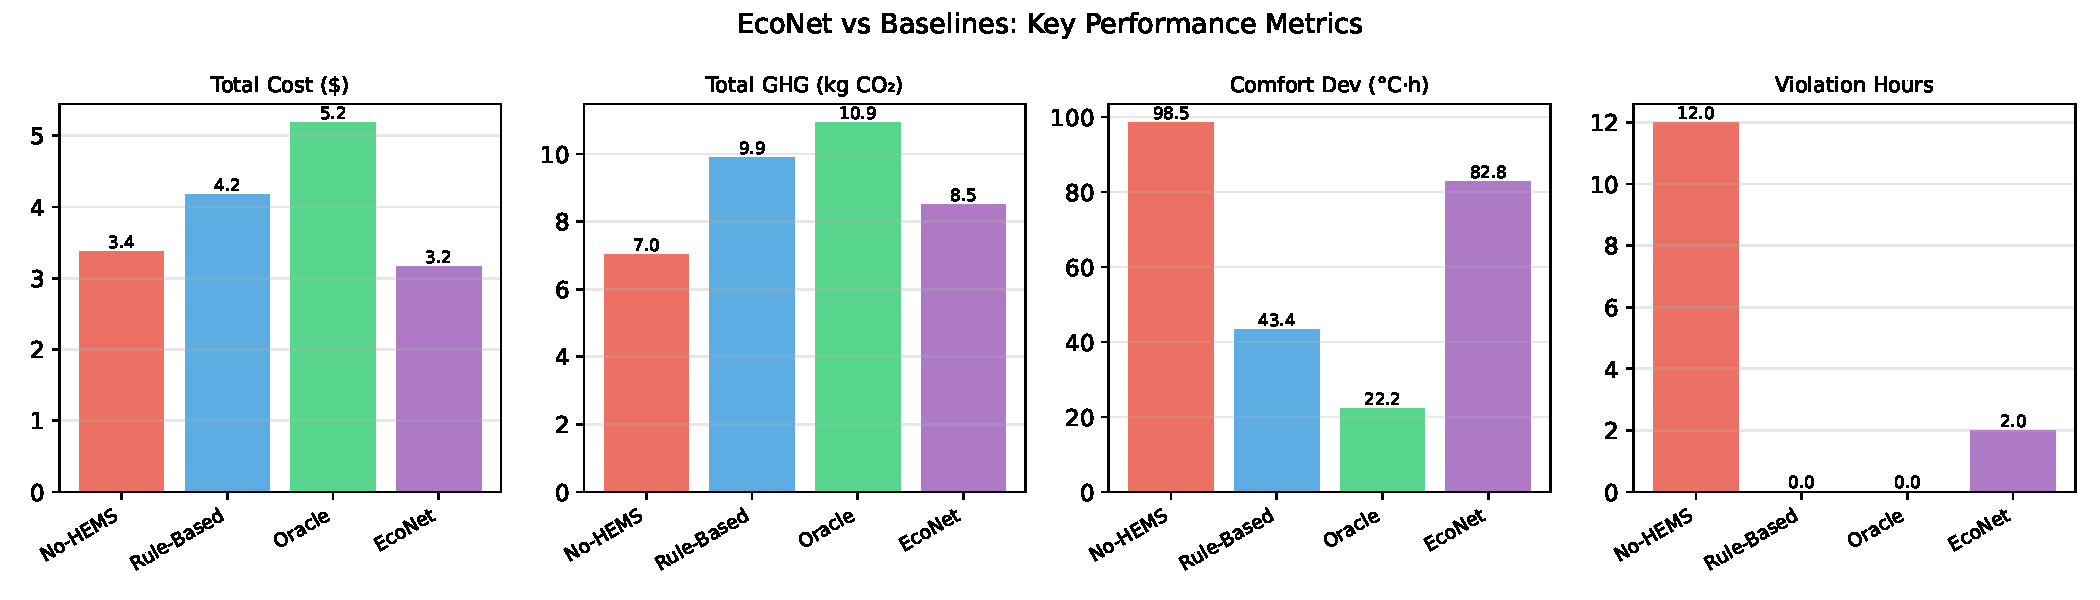
\includegraphics[width=0.85\columnwidth]{figures/baseline_comparison}
\par\end{centering}
\caption{Baseline comparison: daily cost and GHG emissions for EcoNet, No-HEMS,
and Rule-Based controllers.}\label{fig:baseline_comparison}
\end{figure}


\subsection{Climate Sensitivity Analysis}\label{sec:climate}

A key question for any HEMS approach is whether it generalizes across
different climate conditions. To investigate this, we run EcoNet using
real hourly weather data obtained from the Iowa Environmental Mesonet
(IEM) Automated Surface Observing System (ASOS) network for four
geographically diverse cities: London (UK), Phoenix (USA), Montreal
(Canada), and Miami (USA).\footnote{Cities were selected to span four
distinct climate zones: maritime temperate (London), hot arid (Phoenix),
cold continental (Montreal), and tropical humid (Miami). This captures
the major thermal stress regimes relevant to residential HVAC.} For each city, we simulate both a representative
summer week and a representative winter week. We evaluate both the
Aligned coordination mode and the ToM+Belief mode on all eight scenarios
to assess whether belief sharing generalizes across climates.

The grid emission factors are adapted to reflect regional electricity
generation mixes: Montreal's hydro-dominated grid has substantially
lower emissions per kWh than the fossil-heavy grids serving Phoenix
and Miami. ToU rate schedules are adapted to reflect typical utility
pricing in each region.

Table \ref{tab:climate} presents the results for both coordination modes.
Several patterns emerge. First, winter scenarios consistently show higher
costs and emissions than summer, primarily due to increased heating demand.
Second, Montreal shows dramatically lower GHG emissions despite moderate
costs, reflecting the low carbon intensity of hydroelectric generation.
Third, Phoenix summer shows high emissions due to the energy-intensive
cooling demands combined with a fossil-heavy grid. Fourth, the ToM+Belief
mode achieves cost and GHG reductions in six of eight scenarios compared
to Aligned, with an aggregate reduction of 0.6\% in cost and 0.6\% in
GHG emissions. The comfort trade-off is modest (+2.1\% aggregate),
consistent with the cost-comfort Pareto trade-off observed in the synthetic
experiments (Section \ref{sec:coordination_results}). Notably, neither mode requires any retraining or parameter adjustment
between scenarios. The same generative model structure adapts to each
environment through its belief updating mechanism.

\begin{table}[htbp]
\centering
\caption{Climate sensitivity results using real weather data from four cities.
Both Aligned and ToM+Belief coordination modes are evaluated on all scenarios.}\label{tab:climate}
\begin{tabular}{llcccccc}
\toprule
& & \multicolumn{3}{c}{\textbf{Aligned}} & \multicolumn{3}{c}{\textbf{ToM+Belief}} \\
\cmidrule(lr){3-5} \cmidrule(lr){6-8}
\textbf{City} & \textbf{Season} & \textbf{Cost} & \textbf{GHG} & \textbf{Comf.} & \textbf{Cost} & \textbf{GHG} & \textbf{Comf.} \\
& & \textbf{(\$)} & \textbf{(kg)} & \textbf{($^\circ$C$\cdot$h)} & \textbf{(\$)} & \textbf{(kg)} & \textbf{($^\circ$C$\cdot$h)} \\
\midrule
London & Summer & 14.40 & 26.74 & 144.6 & 14.13 & 26.31 & 159.2 \\
London & Winter & 35.70 & 63.57 & 139.4 & 35.58 & 63.32 & 139.4 \\
Phoenix & Summer & 18.46 & 50.48 & 196.3 & 18.46 & 50.48 & 196.3 \\
Phoenix & Winter & 16.93 & 50.96 & 125.7 & 16.32 & 49.79 & 143.0 \\
Montreal & Summer & 8.76 & 3.56 & 137.5 & 8.68 & 3.54 & 137.5 \\
Montreal & Winter & 18.38 & 7.77 & 130.3 & 18.32 & 7.75 & 130.3 \\
Miami & Summer & 20.60 & 69.08 & 261.6 & 20.94 & 69.48 & 256.3 \\
Miami & Winter & 17.78 & 59.80 & 152.7 & 17.64 & 59.20 & 152.7 \\
\midrule
\multicolumn{2}{l}{\textit{Mean}} & 18.88 & 41.50 & 161.0 & 18.76 & 41.23 & 164.3 \\
\bottomrule
\end{tabular}
\end{table}

Figure \ref{fig:climate_real} visualizes the side-by-side comparison
of both modes across all eight scenarios, and Figure \ref{fig:7day_real}
shows the extended 7-day simulation traces for London summer under the
ToM+Belief mode, illustrating how the agent's battery scheduling adapts
to day-to-day weather variability while incorporating the partner agent's
shared beliefs.

\begin{figure}
\begin{centering}
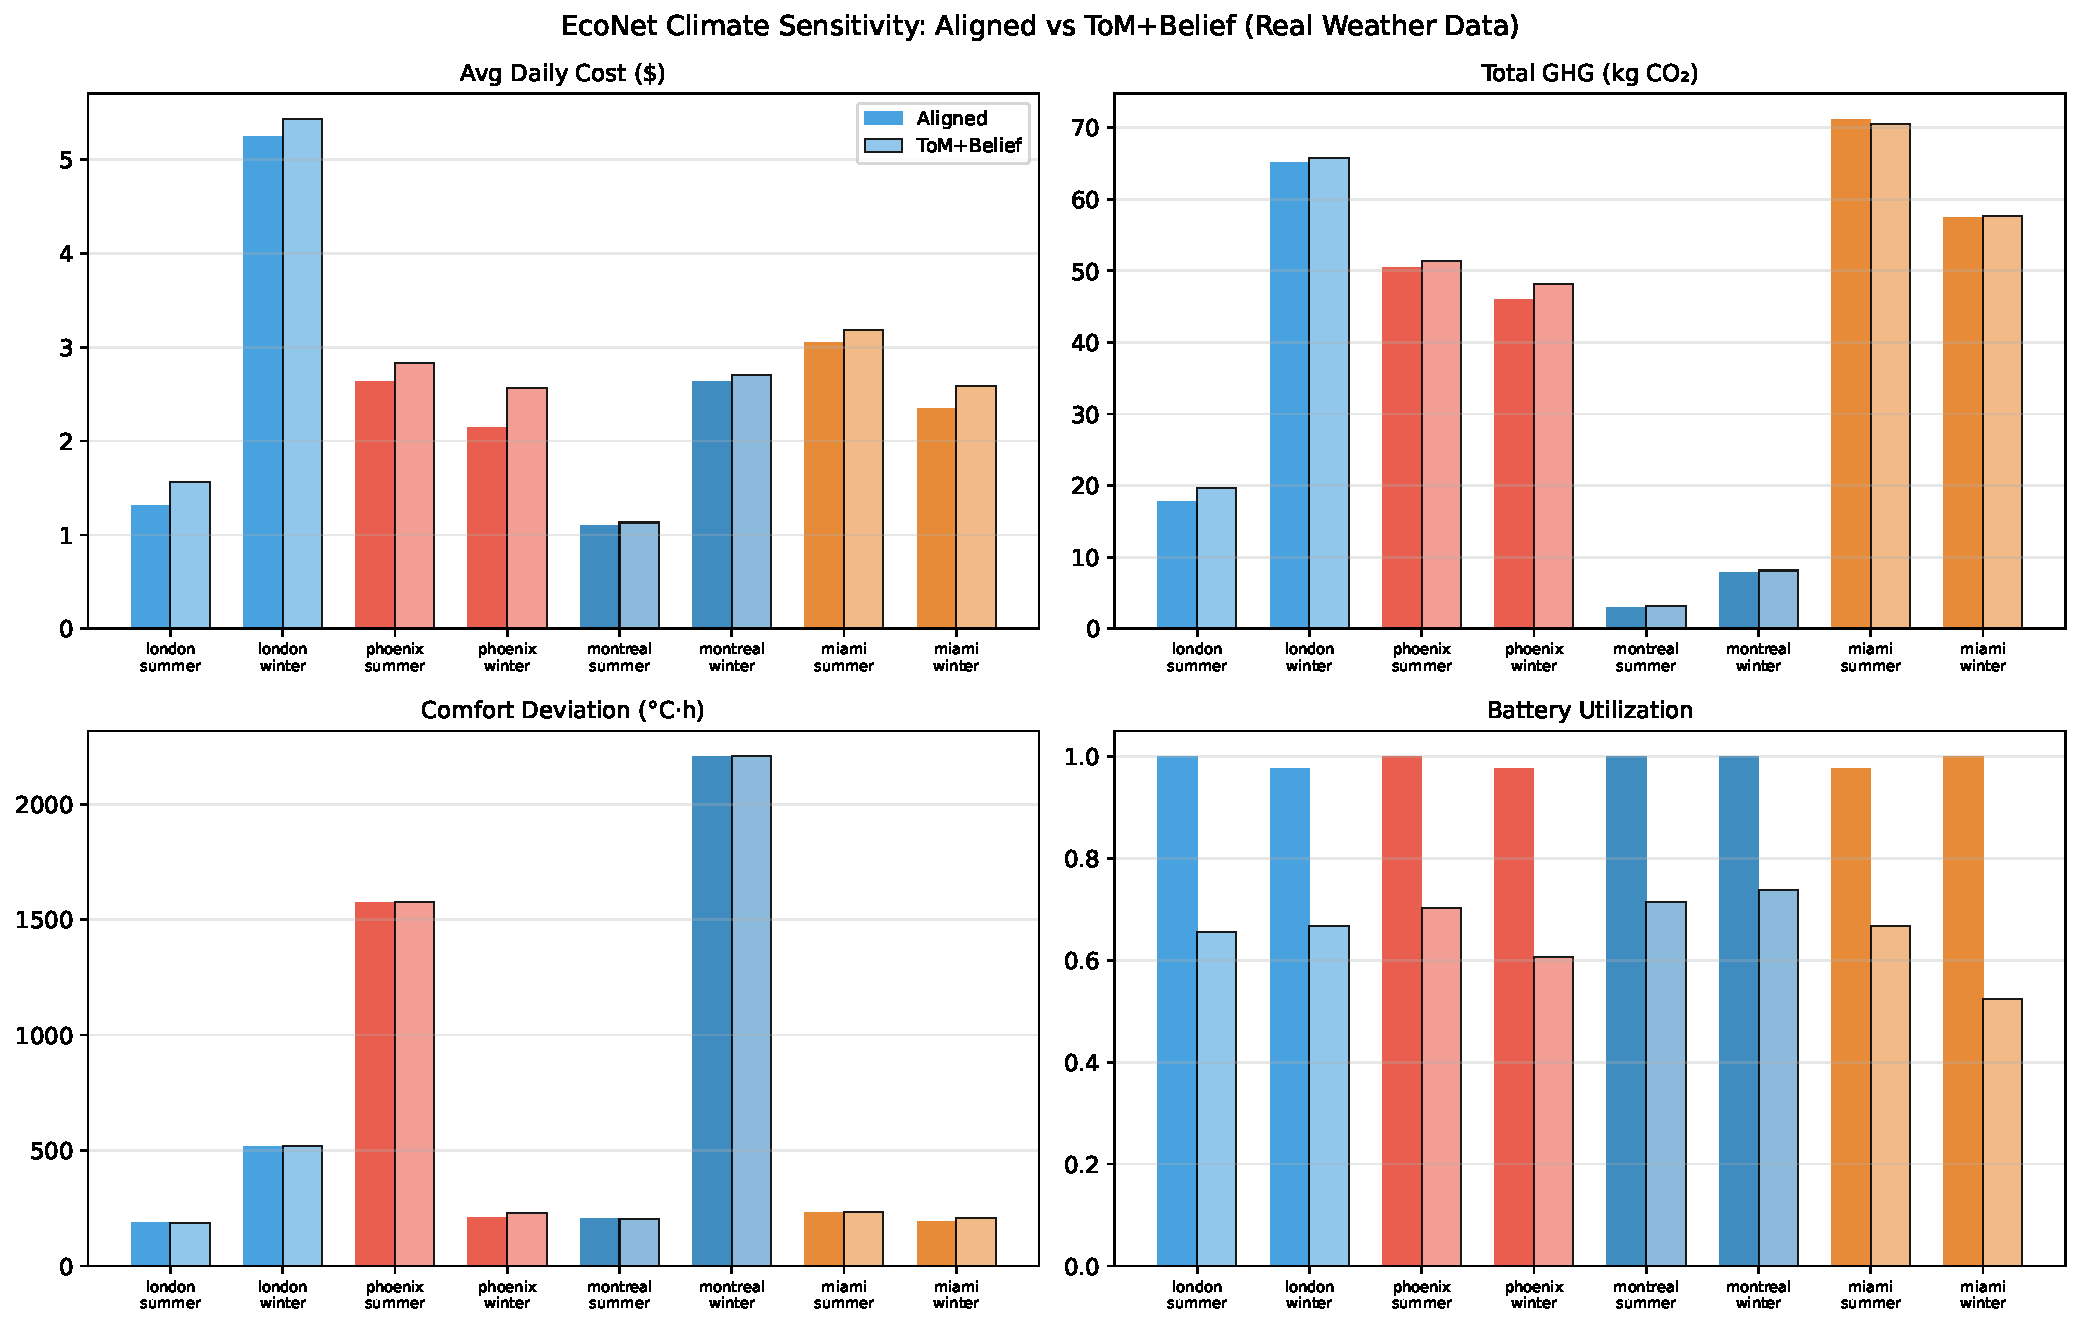
\includegraphics[width=0.95\columnwidth]{figures/fig13_climate_real_weather}
\par\end{centering}
\caption{Climate sensitivity analysis with real weather data: Aligned vs
ToM+Belief across four cities and two seasons. ToM+Belief achieves comparable
or slightly lower cost and GHG in most scenarios.}\label{fig:climate_real}
\end{figure}

\begin{figure}
\begin{centering}
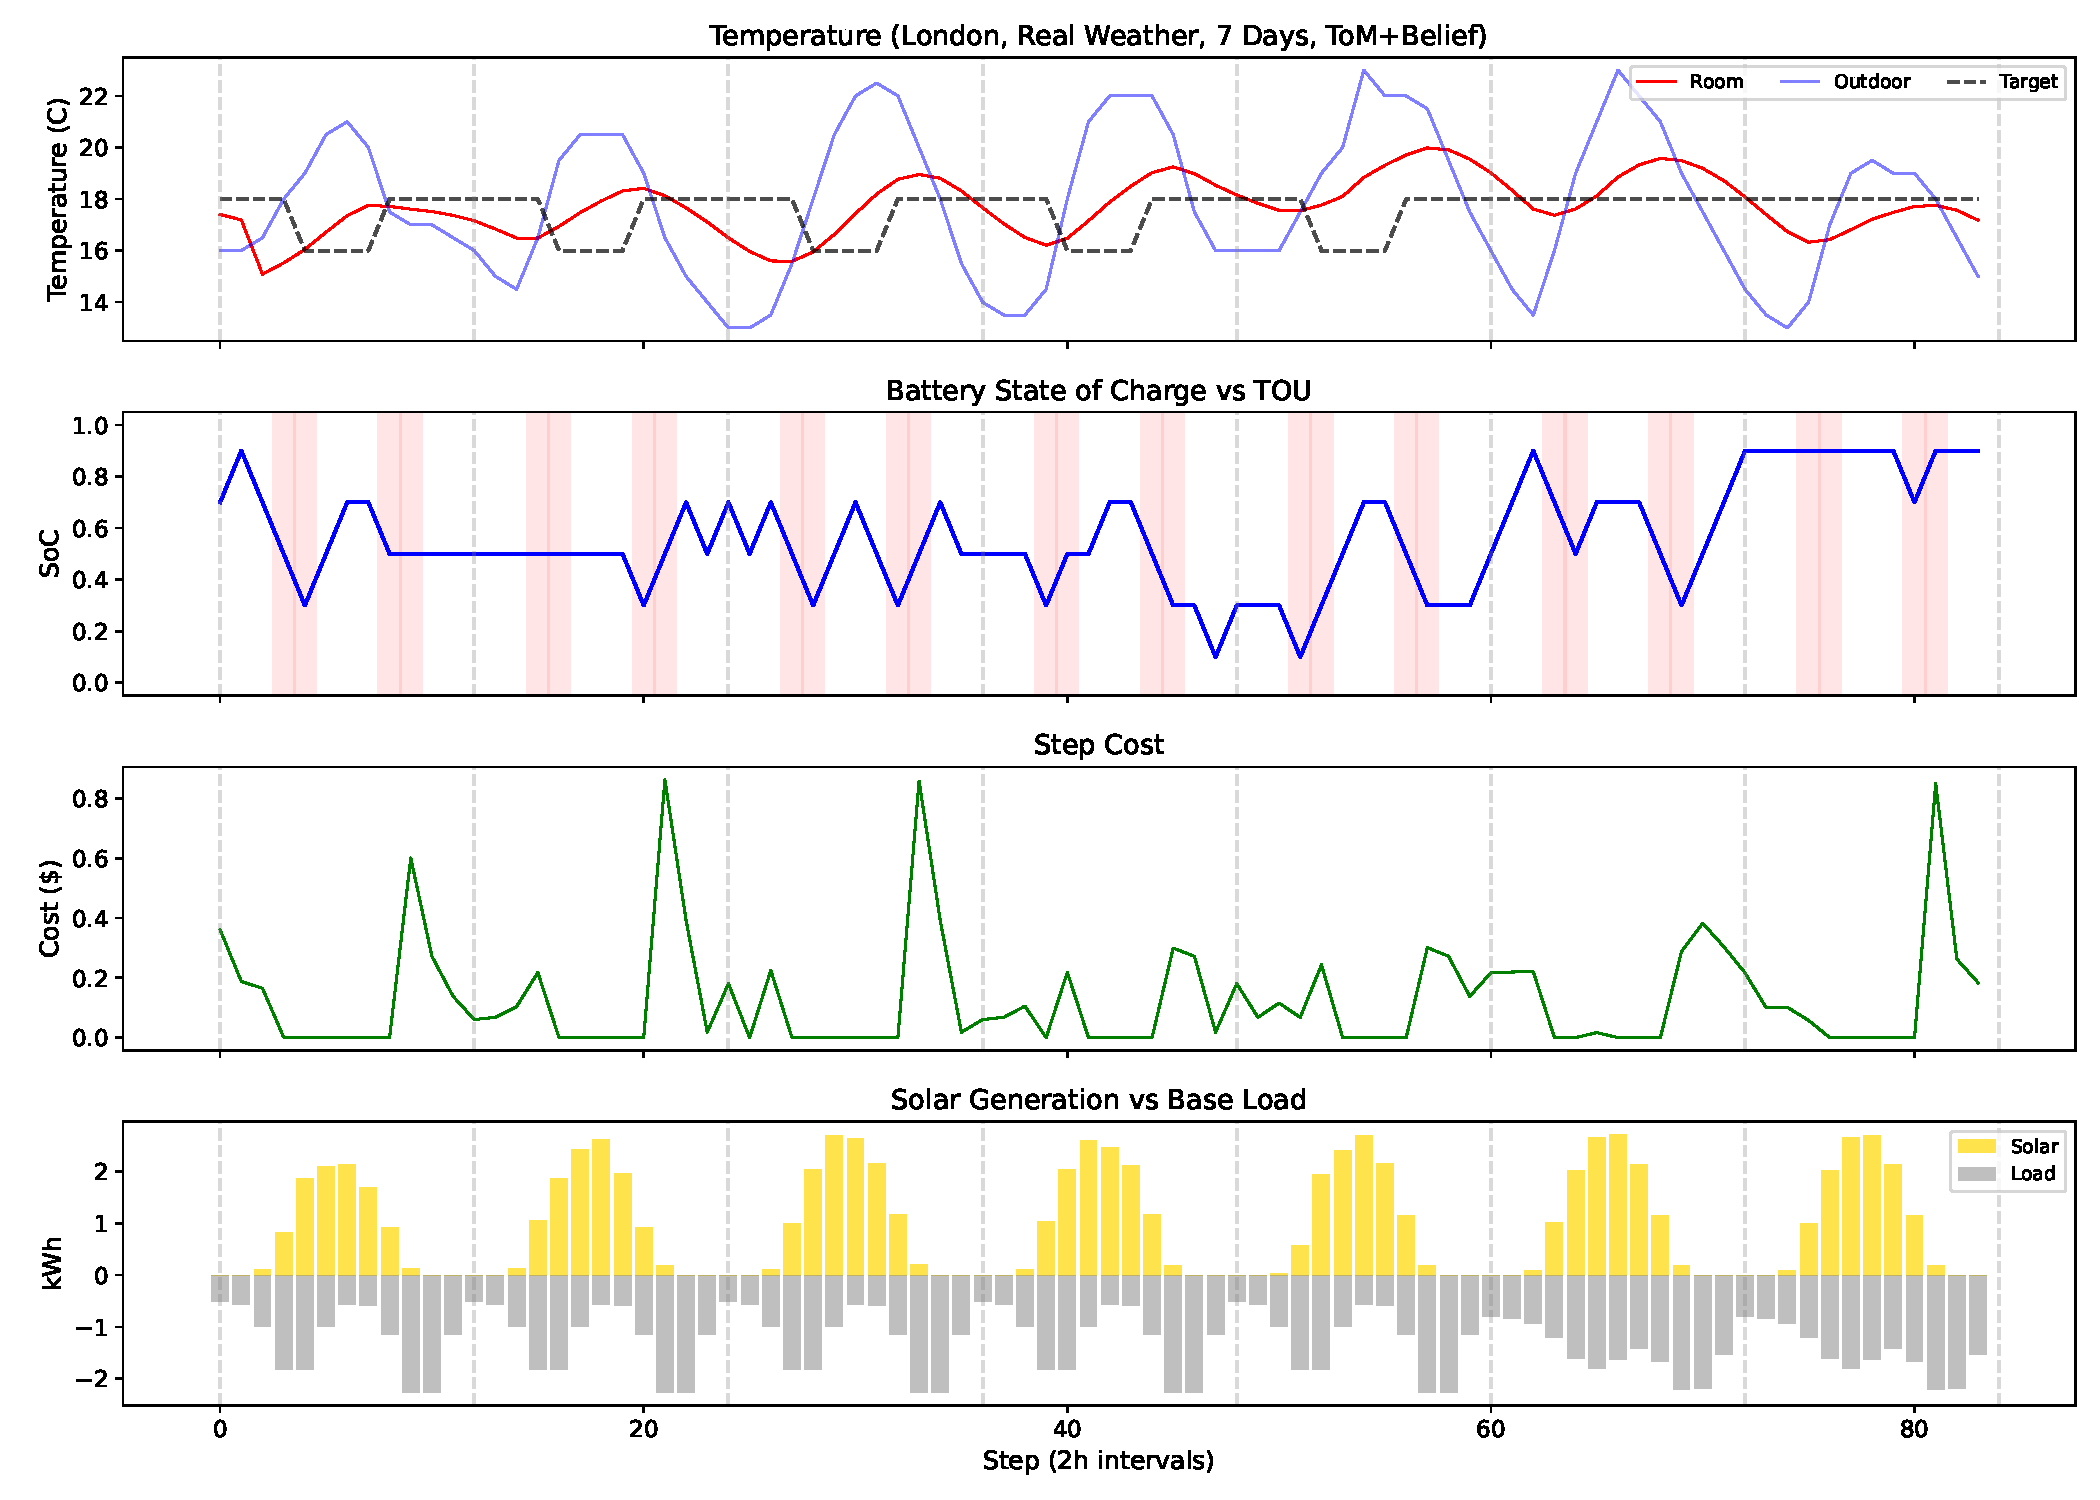
\includegraphics[width=0.85\columnwidth]{figures/fig14_extended_real_weather}
\par\end{centering}
\caption{Extended 7-day simulation with real weather data (London summer,
ToM+Belief mode) showing temperature tracking, battery SoC, cost, and
solar/load profiles.}\label{fig:7day_real}
\end{figure}

We also conducted climate sensitivity experiments using synthetic but
climate-representative weather profiles (Figure \ref{fig:climate_synthetic}).
Results are qualitatively consistent with the real-weather analysis,
confirming that synthetic data can serve as a reasonable proxy for
initial system evaluation. Figure \ref{fig:7day_synthetic} shows the
corresponding extended 7-day simulation with synthetic weather inputs.

\begin{figure}
\begin{centering}
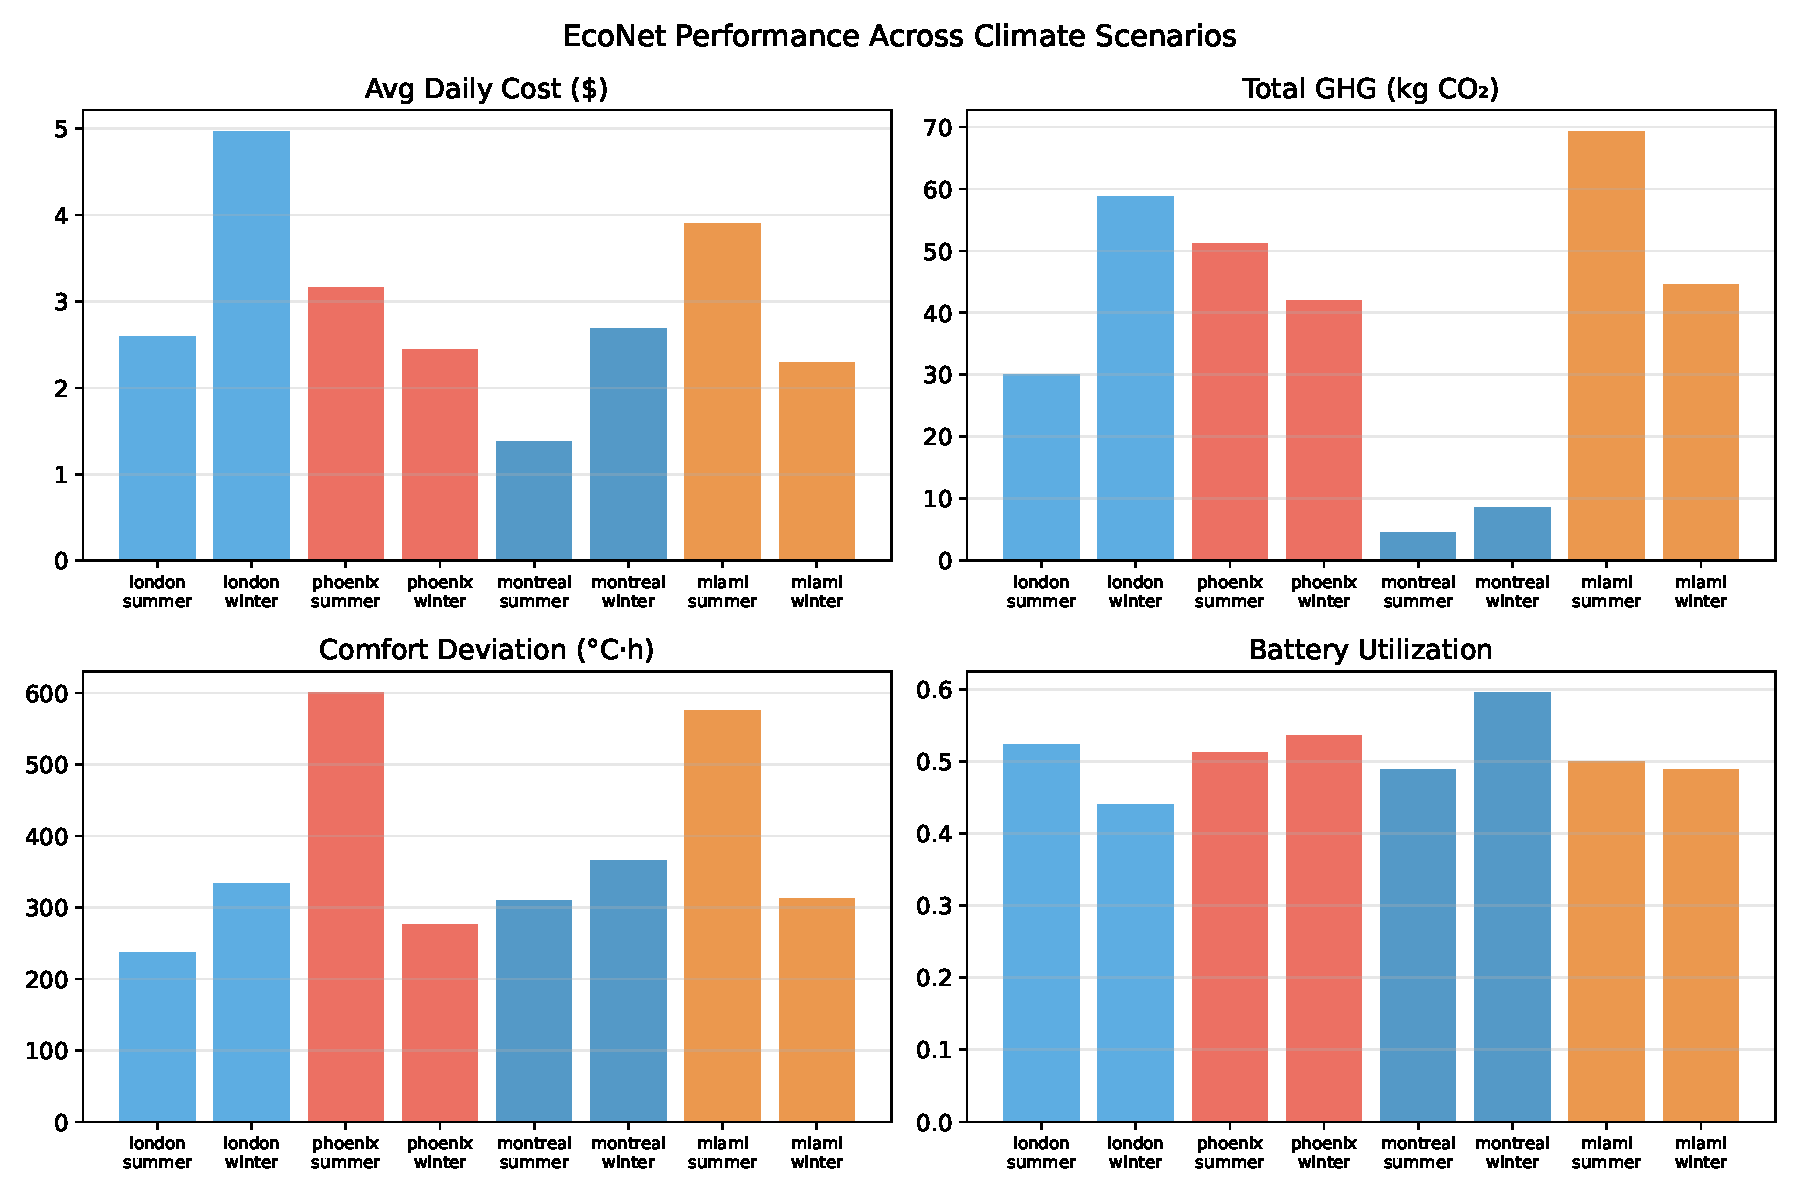
\includegraphics[width=0.85\columnwidth]{figures/climate_sensitivity_synthetic}
\par\end{centering}
\caption{Climate sensitivity analysis with synthetic weather profiles for four
cities across two seasons.}\label{fig:climate_synthetic}
\end{figure}

\begin{figure}
\begin{centering}
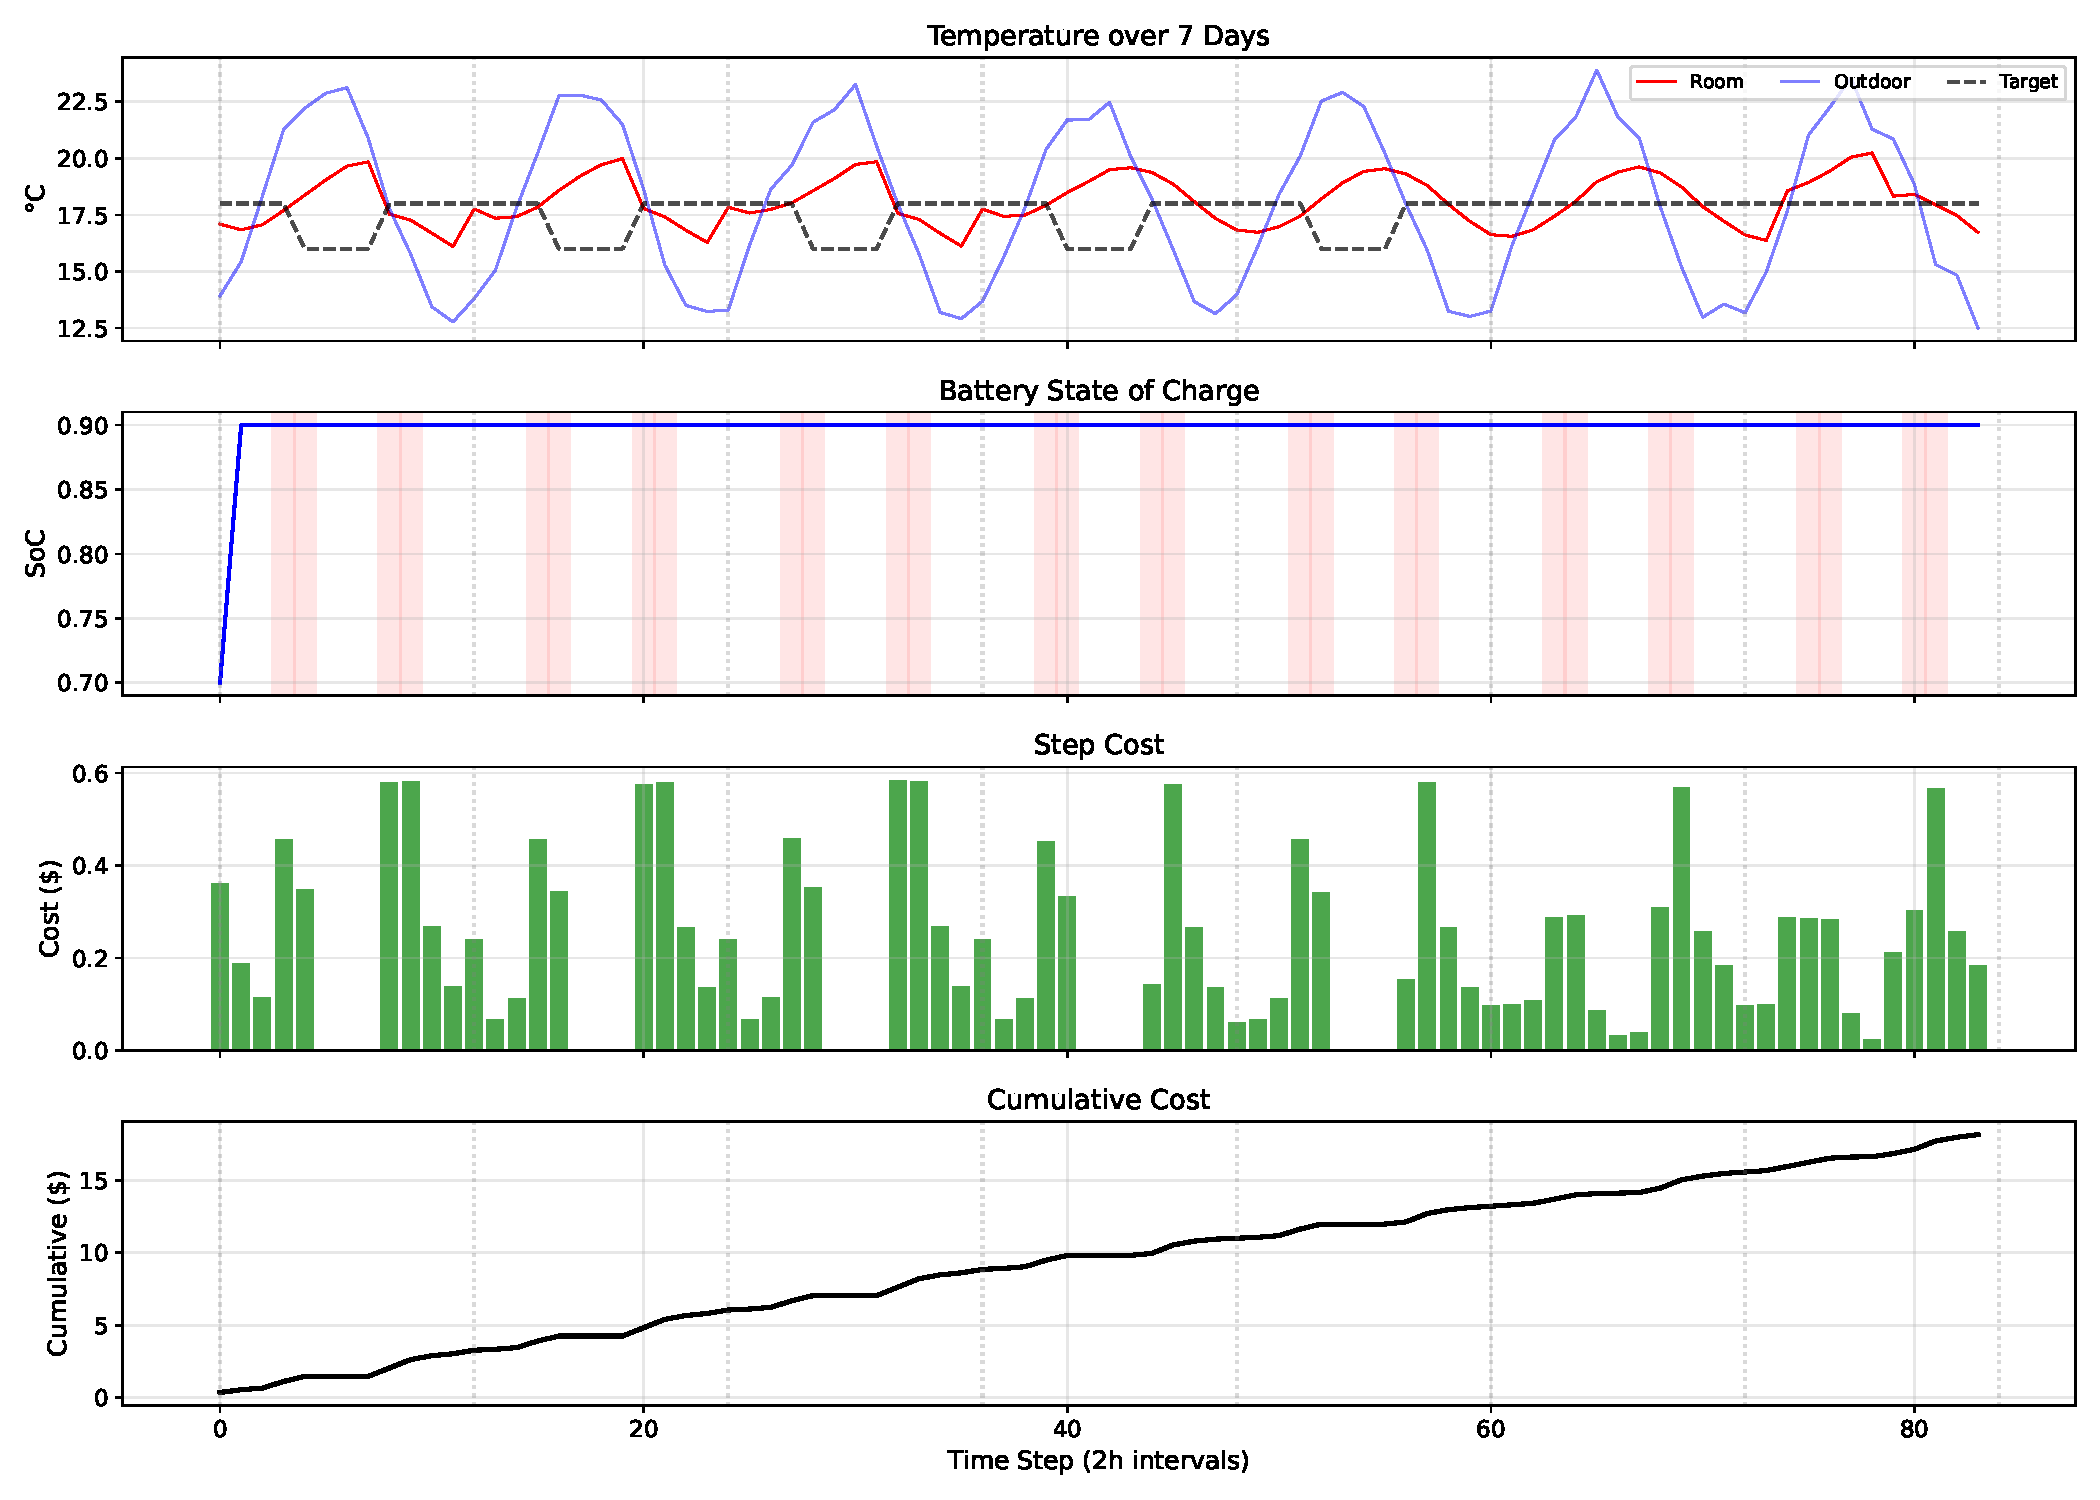
\includegraphics[width=0.85\columnwidth]{figures/extended_7day_synthetic}
\par\end{centering}
\caption{Extended 7-day simulation with synthetic weather profiles.}\label{fig:7day_synthetic}
\end{figure}


\subsection{Validation}\label{sec:validation}

To ensure that the simulation results are physically meaningful, we
perform several validation checks.

\textbf{Energy balance conservation.} At each simulation step, we verify
that total energy equals the sum of baseline load, HVAC energy, battery
energy (positive for charge, negative for discharge), and solar generation
(negative). Across all simulations reported in this paper, the energy
balance is satisfied exactly (to machine precision), confirming that
no energy is created or destroyed by the control logic.

\textbf{Thermodynamic consistency.} The room temperature transition
model satisfies basic thermodynamic constraints: (i) when heating is
off and outdoor temperature is below room temperature, the room cools;
(ii) when cooling is off and outdoor temperature is above room temperature,
the room warms; (iii) heating increases room temperature by an amount
proportional to HVAC capacity; and (iv) cooling decreases it similarly.
These constraints are verified at every step.

\textbf{Battery constraint adherence.} The battery never charges above
SoC = 0.8 or discharges below SoC = 0.2 in any simulation. These
hard constraints are enforced in the generative process (environment)
and are respected by the agent's policy selection due to the structure
of the $B$ matrix, which assigns zero probability to transitions
that would violate these bounds.

\textbf{Gamma sensitivity analysis.} The precision parameter $\gamma$
(inverse temperature) in the softmax policy selection
(Equation~\ref{eq:policy_posterior}) controls the degree of
determinism in action selection. Figure \ref{fig:gamma} shows cost
and GHG performance as $\gamma$ varies from 1 to 32. Performance is
relatively stable for $\gamma \geq 4$, with a slight degradation at
$\gamma = 1$ where the agent's policy selection becomes too stochastic.
The default value of $\gamma = 16$ used throughout this paper sits well
within the stable regime.

\begin{figure}
\begin{centering}
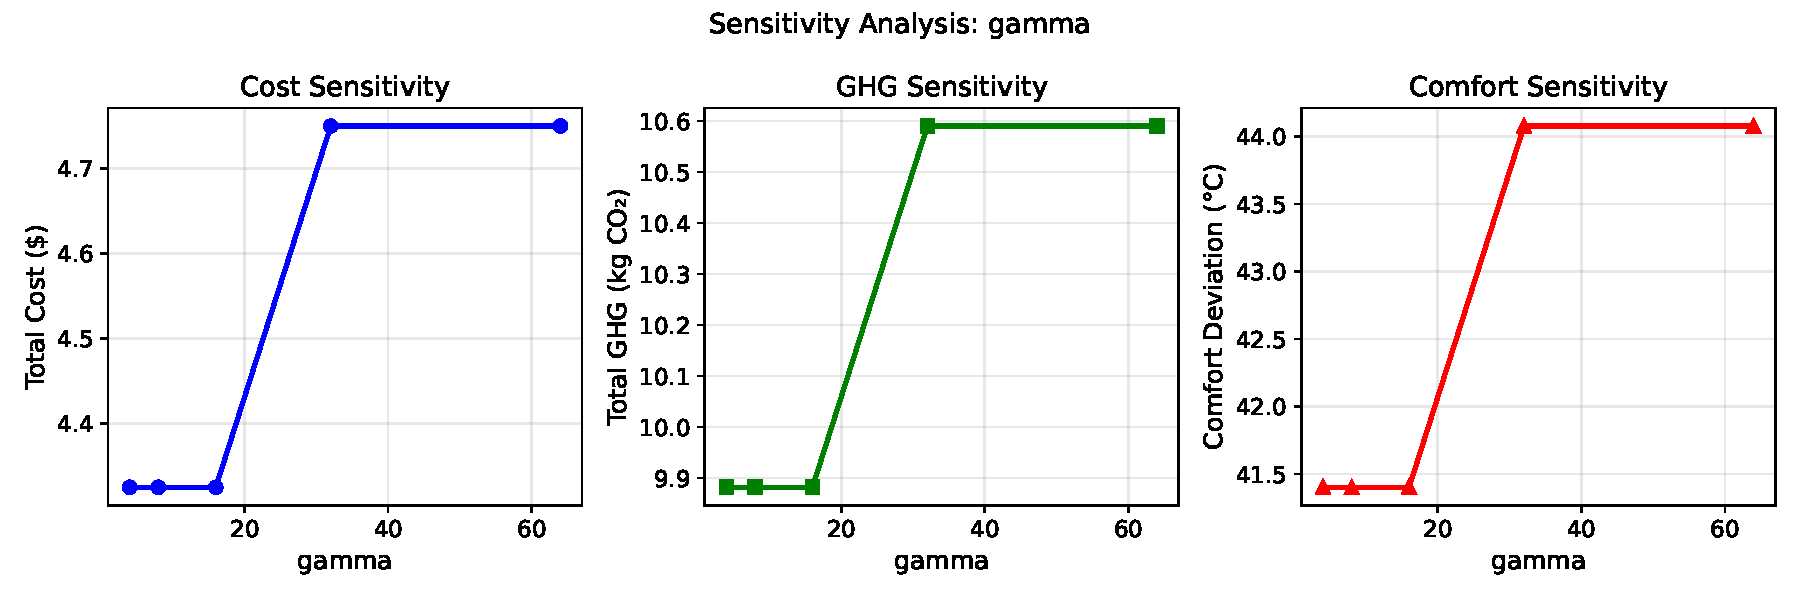
\includegraphics[width=0.85\columnwidth]{figures/gamma_sensitivity}
\par\end{centering}
\caption{Gamma (precision) sensitivity analysis showing cost and GHG emissions
as a function of the softmax inverse temperature parameter.}\label{fig:gamma}
\end{figure}


\subsection{Coordination Mode Comparison}\label{sec:coordination_results}

We compare the coordination modes described in
Section~\ref{sec:coordination} over a 7-day London summer simulation,
averaged over 5 random seeds (policy length 4, $\gamma = 16$,
$B$-learning disabled, predictive $B$ matrices enabled). The Oracle
(backward induction with perfect foresight), MPC (rolling-horizon
backward induction), and tabular RL baselines are included alongside
the non-active-inference baselines. The Sophisticated mode
is evaluated separately in Section~\ref{sec:cost_aware_results}.

Table~\ref{tab:coordination} summarizes the results.
Several patterns emerge. First, all active inference modes achieve
comfort comparable to the No-HEMS deadband thermostat
(${\sim}110$~$^{\circ}$C$\cdot$h), confirming that the $C$~vector
preference structure effectively controls HVAC. The Oracle achieves
the lowest cost (\$18.14) by optimizing battery scheduling with
perfect foresight, while MPC closely matches it (\$18.44) with the
same limited horizon as the AIF agents.

The Aligned mode achieves \$18.90 (4.2\% above Oracle), demonstrating
that the active inference agent approaches optimal battery scheduling
through its generative model. The ToM+Belief mode further reduces cost
to \$18.37 (1.3\% above Oracle), a 2.8\% improvement over Aligned.
This improvement, illustrated in the Pareto frontier of
Figure~\ref{fig:pareto}, arises because belief sharing enables
the Battery Agent to anticipate HVAC demand and time its
charge/discharge decisions accordingly.
The tabular RL baseline performs poorly (\$27.69, 53\% above Oracle)
with substantially degraded comfort (397.9~$^{\circ}$C$\cdot$h),
reflecting the challenge of learning effective energy management
policies from scratch.

\begin{table}[htbp]
\centering
\caption{Coordination mode comparison over a 7-day London summer
simulation, averaged over 5 random seeds.}\label{tab:coordination}
\begin{tabular}{lccc}
\toprule
\textbf{Strategy} & \textbf{Cost (\$)} & \textbf{Comfort ($^{\circ}$C$\cdot$h)} & \textbf{GHG (kg CO$_2$)} \\
\midrule
No-HEMS (baseline) & 22.82 & 112.8 & 37.58 \\
Rule-based          & 19.65 & 112.8 & 34.54 \\
Oracle              & 18.14 & 113.6 & 32.84 \\
MPC                 & 18.44 & 113.6 & 33.19 \\
RL (Q-learning)     & 27.69 & 397.9 & 46.84 \\
EcoNet: Aligned     & 18.90 & 110.5 & 34.44 \\
EcoNet: ToM+Belief  & 18.37 & 108.1 & 33.57 \\
\bottomrule
\end{tabular}
\end{table}

\begin{figure}[htbp]
\begin{centering}
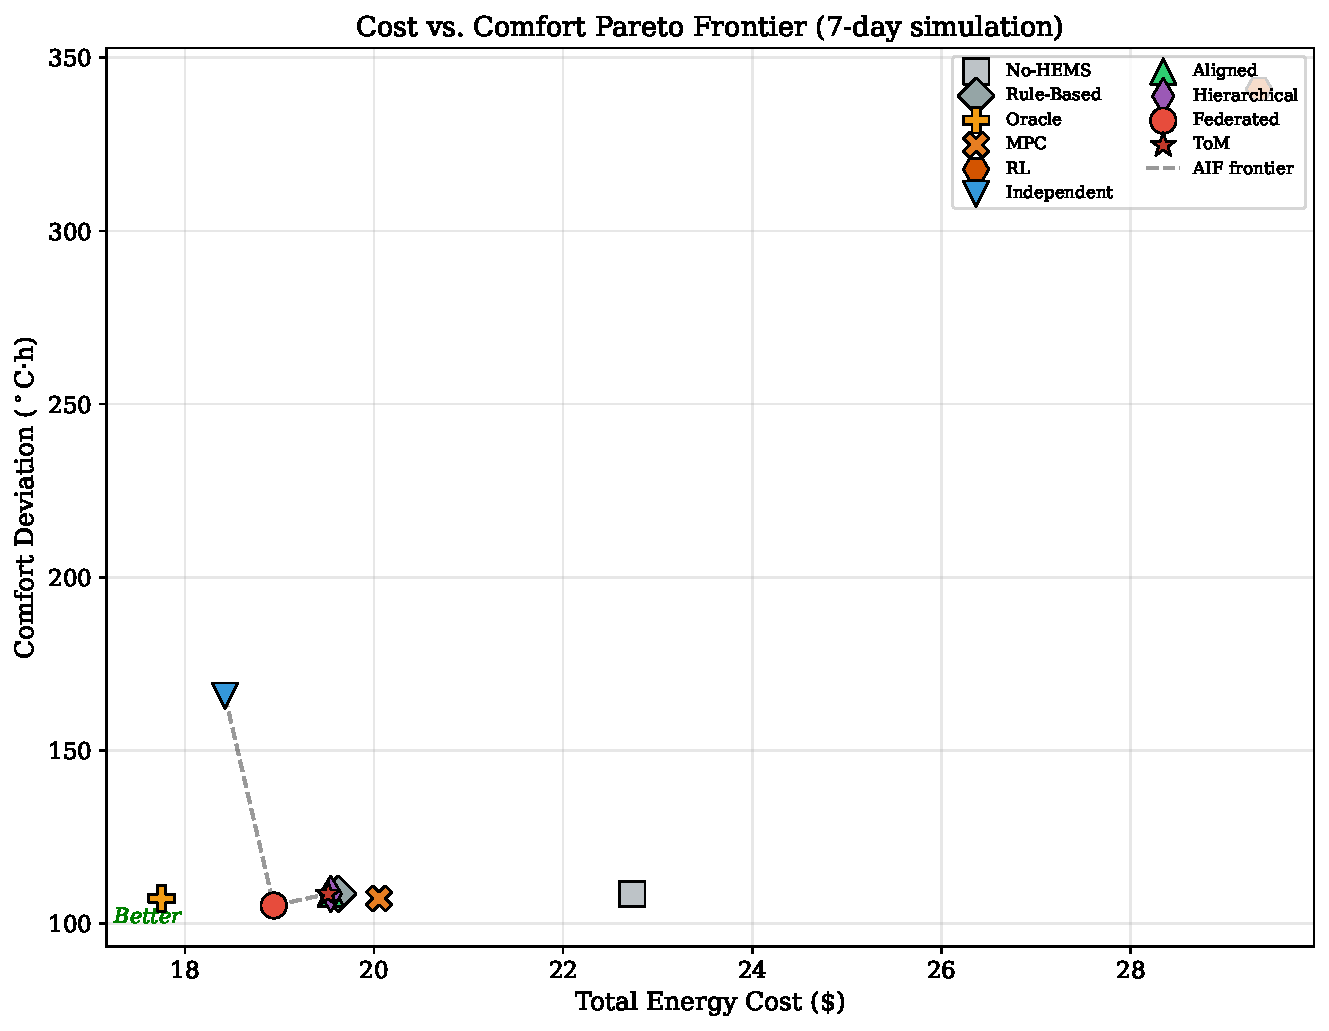
\includegraphics[width=0.85\columnwidth]{figures/fig17_pareto_frontier}
\par\end{centering}
\caption{Cost vs. Comfort Pareto frontier for the first four EcoNet coordination modes
and two baselines. The ToM+Belief mode dominates Aligned on both
cost and comfort.}\label{fig:pareto}
\end{figure}

Figure~\ref{fig:coordination_bars} shows the comparison across all
three key metrics. The No-HEMS baseline has the highest cost (\$22.82)
because its deadband thermostat consumes energy without any battery
optimization to exploit TOU arbitrage. The Oracle achieves the lowest
cost (\$18.14) through perfect-foresight battery scheduling.
Among active inference modes, the Aligned mode (\$18.90, 4.2\% above
Oracle) and ToM+Belief mode (\$18.37, 1.3\% above Oracle) both
achieve near-optimal performance, with ToM+Belief providing the best
comfort (108.1~$^{\circ}$C$\cdot$h) of any condition.
The tabular RL baseline performs worst on both cost (\$27.69) and
comfort (397.9~$^{\circ}$C$\cdot$h).

\begin{figure}[htbp]
\begin{centering}
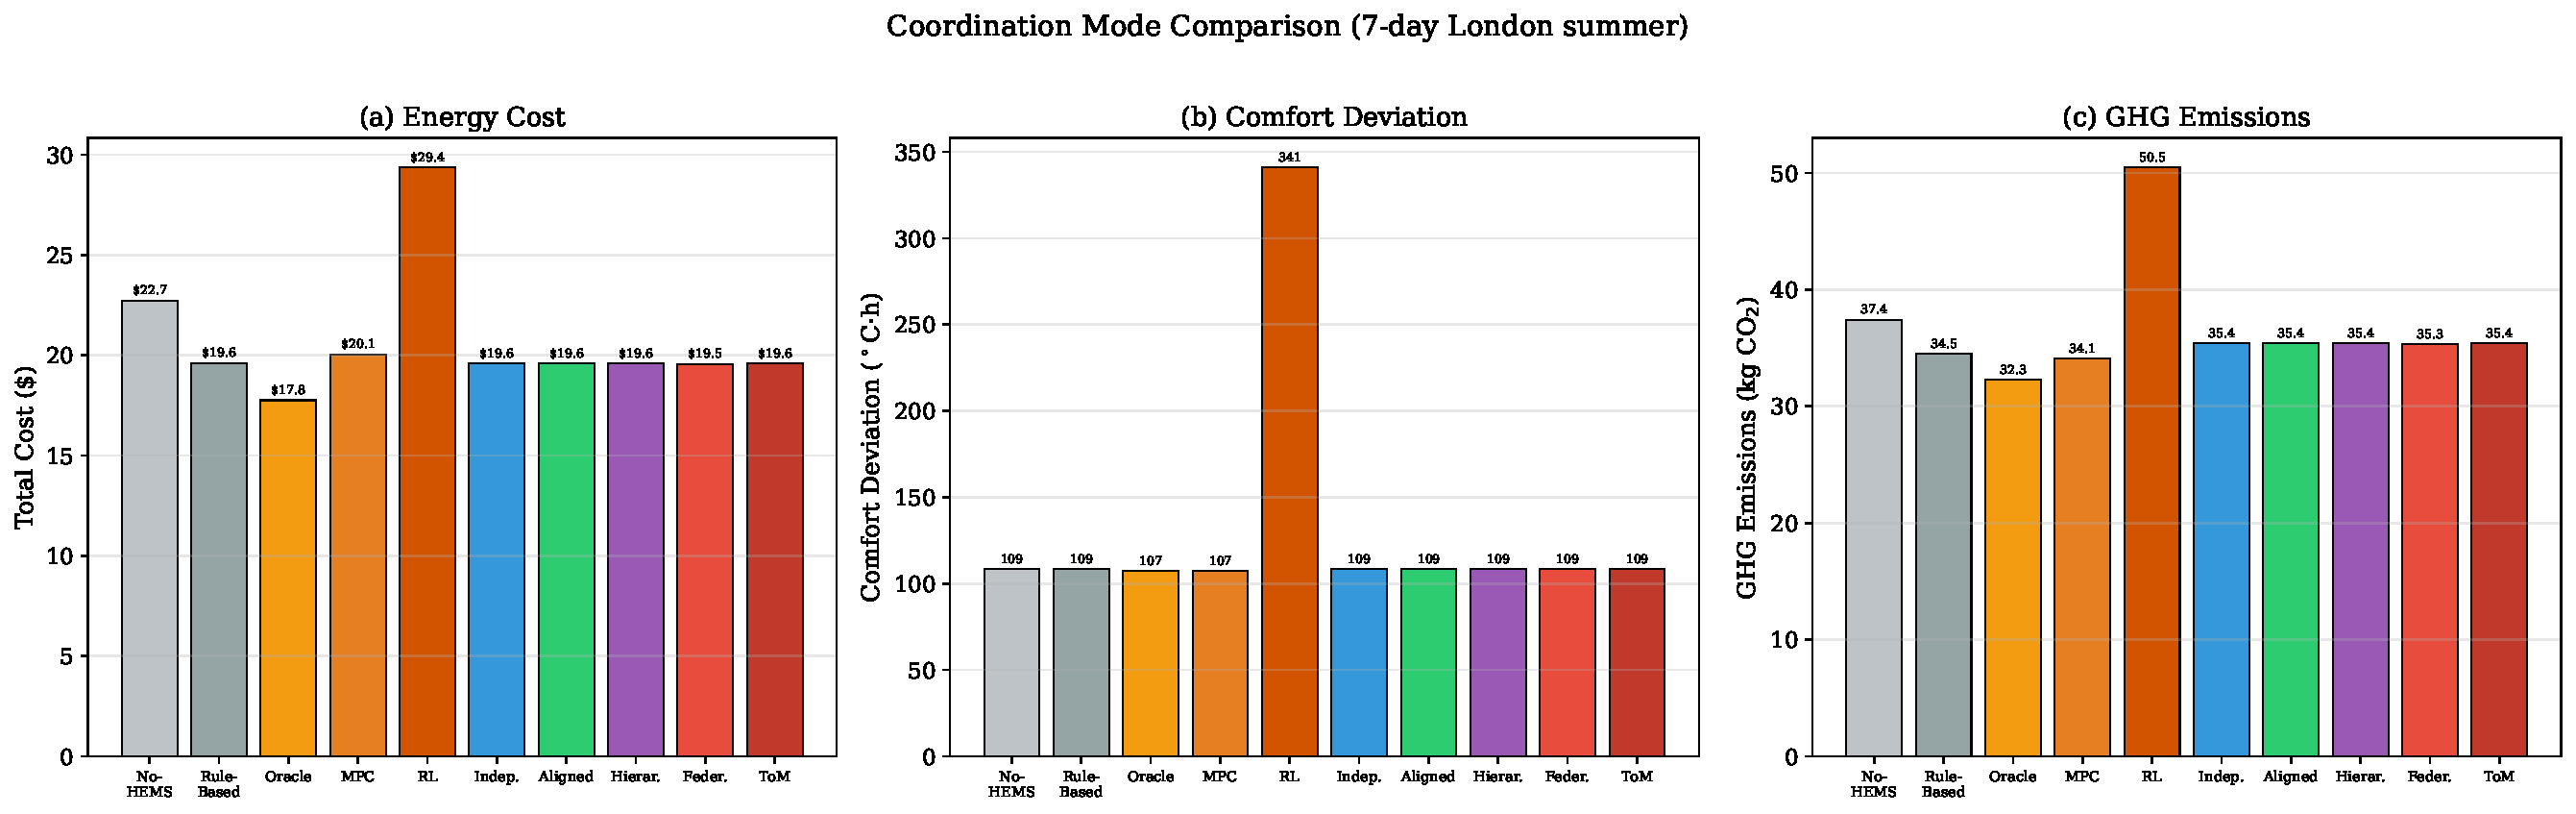
\includegraphics[width=0.95\columnwidth]{figures/fig15_coordination_modes}
\par\end{centering}
\caption{Coordination mode comparison across cost, comfort deviation,
and GHG emissions. Red bars indicate the ToM+Belief mode.}\label{fig:coordination_bars}
\end{figure}

\subsubsection{Belief Sharing Analysis}

The ToM+Belief mode produces rich communication dynamics.
Table~\ref{tab:belief_metrics} reports the key communication metrics.
The average entropy of shared comfort beliefs (0.280~nats) indicates
meaningful uncertainty in the thermostat's comfort assessment, confirming that agents
are genuinely sharing uncertain beliefs, not just relaying point
estimates. Comfort belief diversity of 45.2\% shows that the
thermostat frequently reports non-comfortable states (COLD, COOL,
WARM, or HOT), providing informative signals to the Battery Agent.
The SoC belief diversity of 51.2\% indicates that battery state
varies substantially over the simulation horizon.

Both ToM reliability parameters converge from the initial prior of 0.5
toward higher values (thermostat: 0.728, battery: 0.766), indicating that
each agent learns to trust the other's reports over the 7-day
simulation period (Figure~\ref{fig:tom_reliability}). This
convergence is consistent with the theoretical prediction from
federated inference \cite{friston2024federated}: when agents share
beliefs about a common generative process, their models progressively
align, leading to increasing mutual predictability.

\begin{table}[htbp]
\centering
\caption{Belief sharing metrics for the ToM+Belief mode.}\label{tab:belief_metrics}
\begin{tabular}{lc}
\toprule
\textbf{Metric} & \textbf{Value} \\
\midrule
Avg comfort entropy (nats) & 0.280 \\
Avg SoC entropy (nats) & 0.057 \\
Comfort belief diversity & 45.2\% \\
SoC belief diversity & 51.2\% \\
Thermo ToM reliability (final) & 0.728 \\
Battery ToM reliability (final) & 0.766 \\
\bottomrule
\end{tabular}
\end{table}

\begin{figure}[htbp]
\begin{centering}
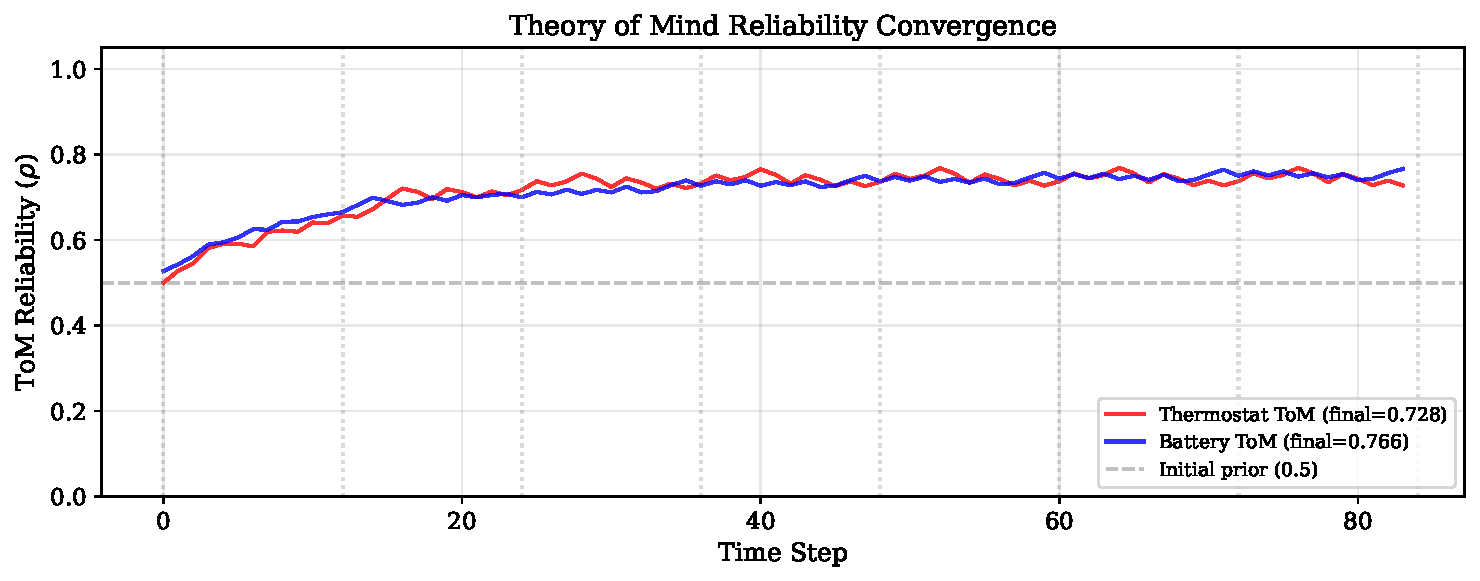
\includegraphics[width=0.85\columnwidth]{figures/fig18_tom_reliability}
\par\end{centering}
\caption{Theory of Mind reliability convergence over the 7-day simulation.
Both agents' ToM reliability parameters ($\rho$) increase from the
uninformative prior of 0.5, indicating that each agent learns to
trust the other's belief reports.}\label{fig:tom_reliability}
\end{figure}


\subsection{Cost-Aware Planning with Predictive Transitions}\label{sec:cost_aware_results}

The final set of experiments evaluates the sophisticated coordination mode
(Section~\ref{sec:cost_aware}), which combines the cost-aware Thermostat
Agent, predictive $B$ matrices for exogenous factors
(Section~\ref{sec:predictive_B}), and mutual phantom inference between
agents. We compare three conditions against an Oracle baseline that uses
backward induction with perfect foresight over the full simulation horizon:

\begin{itemize}
\item \textbf{Aligned}: Standard dynamic $C$ vectors with identity $B$
matrices for exogenous factors (the baseline active inference condition).
\item \textbf{Aligned+Phantom}: The Battery Agent maintains a phantom
Thermostat Agent for HVAC prediction (asymmetric sophisticated inference).
\item \textbf{Symmetric}: Both agents use phantom models of each other.
The Thermostat Agent additionally uses a five-factor generative model
with cost observation, predictive $B$ matrices, and a 12-hour (6-step)
planning horizon.
\end{itemize}

The key architectural difference in the Symmetric condition is
that the Thermostat Agent can now anticipate ToU transitions,
occupancy changes, and outdoor temperature trends through its
predictive $B$ matrices, rather than assuming these factors remain
constant throughout its planning horizon.
The cost-aware generative model enables the Thermostat Agent to reason
about the cost implications of its HVAC decisions by predicting the
Battery Agent's likely response via the phantom battery. At each step,
the phantom battery is queried for its action probability distribution,
which constructs $B_{\text{energy}}$ (Equation~\ref{eq:phantom_B}),
allowing the standard EFE to weigh comfort against cost without any
ad hoc penalty term. The \texttt{cost\_scale} parameter controls the
relative amplitude of $C_{\text{cost}}$ versus $C_{\text{comfort}}$,
producing a smooth Pareto frontier between the two objectives.
A parameter sweep over \texttt{cost\_scale} $\in \{0.5, 1.0, 2.0, 3.0, 5.0\}$
confirms that this frontier is smooth and monotonic, with no abrupt
transitions or performance cliffs.

This combination of predictive exogenous transitions with phantom-mediated
cost awareness represents the most complete instantiation of the active
inference framework for energy management: all relevant information
(tariff schedules, occupancy calendars, weather forecasts, and
inter-agent behavior) enters through the generative model's $B$ matrices
and is evaluated through a single, unmodified EFE objective.

Table~\ref{tab:oracle_gap} reports the Oracle gap analysis across four
climate scenarios over a 7-day simulation with an 8-hour (4-step)
planning horizon and predictive $B$ matrices, averaged over 5 random
seeds. Two additional baselines are included: MPC (rolling-horizon
backward induction with the same 4-step horizon as the AIF agents)
and tabular Q-learning (RL, trained for 500 episodes per seed).
The Oracle uses backward induction with perfect foresight over
the full simulation, providing an upper bound on achievable performance.

\begin{table}[htbp]
\centering
\caption{Oracle gap analysis over a 7-day simulation with policy length 4
(8-hour horizon), predictive $B$ matrices, and $B$-learning disabled.
Results are averaged over 5 random seeds. Gap columns show the
difference relative to the Oracle (positive = worse than Oracle).}\label{tab:oracle_gap}
\begin{tabular}{llcccccc}
\toprule
\textbf{Scenario} & \textbf{Condition} & \textbf{Cost (\$)} & \textbf{Comfort} & \textbf{GHG (kg)} & \textbf{Batt\%} & \textbf{$\Delta$Cost} & \textbf{$\Delta$GHG} \\
\midrule
\multirow{7}{*}{\rotatebox{90}{London summer}}
  & No-HEMS    & 22.82 &  112.8 & 37.58 &   0.0 & $+4.68$ & $+4.74$ \\
  & Rule-based & 19.65 &  112.8 & 34.54 &  51.2 & $+1.51$ & $+1.70$ \\
  & Oracle     & 18.14 &  113.6 & 32.84 &  81.4 & ---     & ---     \\
  & MPC        & 18.44 &  113.6 & 33.19 &  75.7 & $+0.30$ & $+0.35$ \\
  & RL         & 27.69 &  397.9 & 46.84 &  53.1 & $+9.55$ & $+14.00$ \\
  & Aligned    & 18.90 &  110.5 & 34.44 & 100.0 & $+0.76$ & $+1.60$ \\
  & ToM+Belief & 18.37 &  108.1 & 33.57 &  77.6 & $+0.23$ & $+0.73$ \\
\midrule
\multirow{7}{*}{\rotatebox{90}{London winter}}
  & No-HEMS    & 35.69 &  239.8 & 60.99 &   0.0 & $+1.68$ & $+0.09$ \\
  & Rule-based & 35.19 &  239.8 & 60.27 &   2.4 & $+1.18$ & $-0.63$ \\
  & Oracle     & 34.01 &  127.2 & 60.90 &  91.2 & ---     & ---     \\
  & MPC        & 33.78 &  123.7 & 60.29 &  71.7 & $-0.23$ & $-0.61$ \\
  & RL         & 37.29 &  310.2 & 63.87 &  60.2 & $+3.28$ & $+2.97$ \\
  & Aligned    & 34.61 &  108.1 & 61.93 &  94.0 & $+0.60$ & $+1.03$ \\
  & ToM+Belief & 34.46 &  108.1 & 61.61 &  70.2 & $+0.45$ & $+0.71$ \\
\midrule
\multirow{7}{*}{\rotatebox{90}{Montreal winter}}
  & No-HEMS    & 21.13 & 1920.7 &  9.65 &   0.0 & $+2.04$ & $+1.44$ \\
  & Rule-based & 20.86 & 1920.7 &  9.50 &   2.4 & $+1.77$ & $+1.29$ \\
  & Oracle     & 19.09 & 1867.4 &  8.21 &  86.9 & ---     & ---     \\
  & MPC        & 19.12 & 1867.4 &  8.23 &  70.2 & $+0.03$ & $+0.02$ \\
  & RL         & 18.77 & 2937.3 &  8.51 &  51.9 & $-0.32$ & $+0.30$ \\
  & Aligned    & 19.35 & 1867.4 &  8.30 & 100.0 & $+0.26$ & $+0.09$ \\
  & ToM+Belief & 19.51 & 1867.4 &  8.39 &  99.5 & $+0.42$ & $+0.18$ \\
\midrule
\multirow{7}{*}{\rotatebox{90}{Phoenix summer}}
  & No-HEMS    & 27.50 &  853.5 & 63.54 &   0.0 & $+7.79$ & $+9.70$ \\
  & Rule-based & 21.08 &  853.5 & 54.53 &  51.2 & $+1.37$ & $+0.69$ \\
  & Oracle     & 19.71 &  853.5 & 53.84 &  71.2 & ---     & ---     \\
  & MPC        & 19.76 &  853.5 & 54.03 &  71.0 & $+0.05$ & $+0.19$ \\
  & RL         & 26.87 & 1302.2 & 61.54 &  65.7 & $+7.16$ & $+7.70$ \\
  & Aligned    & 19.92 &  853.5 & 54.74 &  70.2 & $+0.21$ & $+0.90$ \\
  & ToM+Belief & 20.51 &  853.5 & 57.34 &  98.8 & $+0.80$ & $+3.50$ \\
\bottomrule
\end{tabular}
\end{table}

Several patterns are notable. First, the Aligned agent closely tracks
the Oracle across all four climates: the average cost gap is \$0.46
(2.0\% of Oracle cost) and the average GHG gap is 0.91~kg (2.3\% of
Oracle GHG), indicating that the predictive $B$ matrices enable the
agent to approach globally-optimal battery scheduling despite having
only an 8-hour rolling horizon. Results are stable across seeds, with
standard deviations of \$0.19--0.64 for AIF cost.

Second, the gap is smallest in the most demanding scenarios. In
Montreal winter, where the extreme cold forces continuous heating
regardless of strategy, the Aligned agent achieves near-Oracle
performance ($\Delta$cost = \$0.26, $\Delta$GHG = 0.09~kg), since the
dominant cost driver (heating) leaves little room for battery
optimization differences. In Phoenix summer, where cooling demand
dominates, the agent again closely tracks the Oracle ($\Delta$cost =
\$0.21), confirming that the generative model adapts to diverse
thermal conditions. The Aligned agent also achieves \emph{better}
comfort than the Oracle in London winter (108.1 vs 127.2~$^{\circ}$C$\cdot$h),
reflecting its strong comfort preference in the $C$ vector.

Third, the No-HEMS baseline (which includes a fixed thermostat
but no battery management) achieves comparable comfort to the active
inference modes, since both use HVAC for temperature control. The
remaining cost gap between No-HEMS and active modes reflects the
value of TOU arbitrage: battery operation incurs round-trip losses
($\eta = 0.9$ one-way, 81\% round-trip), but enables cost savings by
shifting consumption from high-ToU to low-ToU periods that outweigh
these losses. The MPC baseline achieves near-Oracle performance with
the same 4-step horizon as the AIF agents, confirming that the
limited-horizon planning problem is well-conditioned. However, MPC
requires a complete model of system dynamics and deterministic
optimization, whereas the AIF agent learns its generative model
structure and provides uncertainty quantification through posterior
beliefs. The tabular RL baseline performs poorly, with costs 20--53\%
above Oracle and substantially degraded comfort in mild climates,
reflecting the challenge of learning effective policies from scratch
with coarse state discretization.

Fourth, the ToM+Belief mode improves on Aligned in mild climates
(London summer: \$18.37 vs \$18.90, 3\% cost reduction with 2\%
comfort improvement) where the thermostat has meaningful scheduling
choices. In extreme climates (Montreal, Phoenix), where HVAC runs
at capacity regardless, ToM provides no benefit and adds slight
overhead from belief communication.


\section{Discussion}

As societal electrification increases in response to climate change,
and as the penetration of DER devices in distribution grids increases,
it becomes increasingly important for grid flexibility and stability
not only that each energy device is intelligently managed, but that
management is coordinated between devices within a household, between
households of a neighborhood or complex, and across regions of the
grid. Intelligent management involves forecasts (of weather, solar
generation, energy use, household occupancy, etc.) and such forecasts
involve uncertainty. Related, the thermodynamic model of a house is
typically unknown and must be estimated, which also involves uncertainty.
Thus, the use of multi-agent probabilistic models for HEMS appears
promising. In this, the use of active inference seems particularly
promising, as an active inference agent can choose actions to resolve
uncertainty. In an advanced model for example, an agent might ask
a householder if a room will be occupied later in the evening, if
it is unsure. Relatively few HEMS studies conducted so far consider
probabilistic models, however.

Here we demonstrate a proof-of-concept active inference model. Results
suggest that the model is able to plan ahead to balance conflicting
preferences for energy use, energy cost, greenhouse gas emissions,
and comfort. The multi-seed Oracle gap analysis
(Section~\ref{sec:cost_aware_results}) provides the most rigorous
evaluation: across four climate scenarios and five random seeds,
the Aligned agent achieves costs within 2.0\% of the perfect-foresight
Oracle on average, with a maximum gap of 4.2\% (London summer). This
near-optimal performance arises from predictive $B$ matrices that
enable the agent to anticipate environmental changes within its planning
horizon. The cost advantage over a fixed-thermostat baseline (up to 17\%
in mild climates) reflects the value of intelligent battery scheduling
through TOU arbitrage.

The coordination mode comparison (Section~\ref{sec:coordination_results})
reveals several important insights. First, the Aligned mode achieves
costs within 4.2\% of the perfect-foresight Oracle in London summer and
within 1--2\% in extreme climates, demonstrating that the generative model
with predictive $B$ matrices enables near-optimal battery scheduling.
Second, MPC with the same planning horizon achieves near-identical
performance to the AIF agents, confirming that the limited-horizon planning
problem is well-conditioned; the advantage of AIF lies in its probabilistic
framework and uncertainty quantification rather than in raw performance.
Third, the ToM+Belief mode provides modest but consistent improvements
over Aligned in mild climates (3\% cost reduction in London summer),
where the thermostat has meaningful scheduling flexibility. In extreme
climates, where HVAC runs at capacity regardless of strategy, the
benefit vanishes.

This result is consistent with the theoretical prediction from federated
inference \cite{friston2024federated}: sharing posterior beliefs (full
probability distributions, not point estimates) enables agents to form
decentralized consensus about shared world states, with the magnitude
of the benefit depending on the degree of coordination opportunity
in the environment. The auditory A matrix formulation (explained in
Section~\ref{sec:tom_mode} as a likelihood mapping that translates
received beliefs into observation probabilities within the generative
model) ensures that social preferences emerge naturally within the
standard EFE computation (Equation~\ref{eq:social_efe}), requiring no
additional optimization objective or hand-tuned coordination mechanism.
The ToM reliability parameter (Equation~\ref{eq:reliability}) provides a
principled mechanism for trust calibration, allowing agents to discount
unreliable reports, a property that would be essential in real-world
deployment where sensor noise and communication delays are common.

The predictive $B$ matrix approach (Section~\ref{sec:predictive_B})
demonstrates a principled way to incorporate forecast information into
the active inference framework. Rather than treating exogenous state
dynamics as unknown or static, agents update their transition
beliefs using available information---published tariff schedules,
occupancy calendars, and weather forecasts---at each time step. This
is consistent with the active inference principle that an agent should
maintain the most accurate generative model possible: forecast data
simply provides better priors on state transitions. The Gaussian
kernel for outdoor temperature (Equation~\ref{eq:predictive_B_temp})
naturally encodes forecast uncertainty, with the spread parameter
$\sigma$ reflecting confidence in the weather prediction.

The cost-aware planning architecture
(Section~\ref{sec:cost_aware_results}) extends this principle by
introducing inter-agent prediction through phantom models.
The Thermostat Agent's phantom battery provides a probabilistic
forecast of the Battery Agent's behavior, which enters the generative
model as $B_{\text{energy}}$ (Equation~\ref{eq:phantom_B}). This
construction is noteworthy because cost awareness emerges entirely
within the standard EFE framework: no custom objective function or
additive cost penalty is required. The agent simply has a richer
generative model that includes energy demand as a state factor and
cost as an observation, with preferences encoded in the $C$ vector.
The \texttt{cost\_scale} parameter provides a transparent and
interpretable mechanism for trading off comfort against cost,
producing a smooth Pareto frontier without requiring retraining.

From a broader perspective, the five coordination modes map onto a
spectrum from fully decentralized (Independent) to fully centralized
(Hierarchical), with the Aligned, ToM+Belief, and Sophisticated modes
occupying intermediate positions. The ToM+Belief mode, a purely
decentralized architecture, provides modest improvements over the
non-communicating Aligned mode in mild climates where the thermostat
has meaningful scheduling flexibility (3\% cost reduction in London
summer). In extreme climates where HVAC runs at capacity, the
coordination opportunity is limited and ToM provides no benefit.
This environment-dependent benefit suggests that peer-to-peer belief
sharing is most valuable when agents face genuine coordination
dilemmas, consistent with findings on collective active inference,
where ensembles of agents coordinating through shared beliefs can
achieve emergent global behavior
\cite{heins2024collective,heins2023spin}. The
Sophisticated mode offers an alternative path to coordination: rather
than communicating beliefs directly, each agent maintains a phantom
model of the other's decision process and anticipates its behavior.
This can be seen as an implicit form of Theory of Mind that does
not require a communication channel \cite{pitliya2025theory}.

The climate sensitivity analysis (Section~\ref{sec:climate}) demonstrates
that EcoNet generalizes across diverse climate conditions without
retraining---a direct consequence of active inference's online adaptation
through belief updating, in contrast to RL approaches that would require
re-training for each new climate. The agent adapts its behavior---for
example, prioritizing cooling in Phoenix summers and heating in Montreal
winters---through the standard belief-updating mechanism of active inference. The use of
real weather data from the IEM ASOS network provides confidence that
performance would be maintained under realistic operating conditions.

The validation results (Section~\ref{sec:validation}) confirm that
the simulation framework maintains physical consistency. This is
important because energy management systems that violate conservation
laws or constraint boundaries in simulation cannot be trusted for
deployment. The gamma sensitivity analysis further shows that performance
is robust to the choice of precision parameter within a reasonable
range.

Multiple studies suggest that HEMS and related energy management systems
have potential to reduce energy costs, conserve resources, reduce
greenhouse gas emissions, and increase grid stability and function
\cite{khabbazi2025,Mahapatra2022-zp,Martinez-2021,Tuomela-2021}.
To highlight one example, Gualandri and Kuzior \cite{Gualandri-2023}
demonstrate that increased adoption of HEMS could dramatically reduce
residential-energy consumption in Italy, which in their view could
help the country to achieve 2030 European energy targets. The degree
of future HEMS adoption depends of course on choices made by manufacturers,
utilities, consumer groups, end users, policymakers, and other stakeholders,
which in turn depends on the degree of cooperation between these entities
\cite{oluokun-2025,land14030566,Khafiso-2024}.

\subsection{Limitations}

Several limitations of the current study should be acknowledged.
First, the 2-hour time step discretization limits the model's ability
to capture fast dynamics such as HVAC cycling or sub-hourly TOU tariffs.
Finer temporal resolution would increase the state space and planning
horizon, potentially requiring approximate inference methods.
Second, the $B$ matrices for exogenous factors (outdoor temperature,
occupancy, TOU) are currently rebuilt from known schedules and forecasts
at each step; in a real deployment, forecast uncertainty would grow
with the prediction horizon and should be modeled explicitly.
Third, the coordination mode comparison uses a single seed for the
7-day simulation; while the results are consistent across the 2-day
and climate sensitivity analyses, multi-seed experiments with
confidence intervals would strengthen the statistical conclusions.
Finally, the symmetric sophisticated mode (Section~\ref{sec:cost_aware_results})
is computationally expensive due to the expanded policy space ($3^6 = 729$
policies with 5 state factors), and we were unable to run it for the full
7-day duration on all climate scenarios. Computational optimization
(e.g., policy pruning, amortized inference) would be needed for
practical deployment.

\subsection{Future Work}

There are many possibilities for future work that could extend or
improve upon the current model. Like Nazemi et al. we could employ
a continuous state space and test the model using data generated from
real buildings or accurate digital twins. Although our aim is to coordinate
energy management across households, the current model only considers
management within a single building. Extension to neighborhoods or
building clusters would naturally expand our two-agent model to a
many-agent approach. The belief-sharing architecture presented here
provides a natural foundation for such scaling, as each agent need only
communicate with its immediate neighbors rather than a central coordinator
\cite{friston2024federated}. While our predictive $B$ matrices already
incorporate weather forecasts and known schedules, future efforts could
extend this to fully probabilistic multi-step forecasts, where forecast
uncertainty grows with the prediction horizon. More efficient methods for parameter and
structure learning are also possible, especially for learning complex
thermodynamic models of buildings. Renormalization group models or
tensor networks could be interesting here due to their capacity to
capture scale-invariance and compress data associated with high dimensional
functions, including probability functions \cite{Friston-2025,Roa-2024}.
The ToM reliability mechanism could be extended to learn the auditory
A matrix itself, allowing agents to adaptively model each other's
communication patterns, a form of hierarchical active inference
\cite{pezzulo2018hierarchical,poppel2022resonating} applied to
social cognition.
Finally, it would be interesting to apply an active inference model
to infer the goals, preferences, and beliefs of households that largely
determine how they manage their energy devices. For example, a solar
battery inverter can be managed in numerous ways, for numerous purposes,
each of which could alter the voltages, currents, and power factors
seen at the point of common coupling with the grid. Given a history
of device management, as evidenced by the numerical readings available
to grid operators, what model best explains the management practices
of a household, and so also its expected energy impacts on the grid?

\section{Conclusion}

We have presented EcoNet, a multi-agent active inference framework for
household energy management that unifies perception, planning, learning,
and coordination under the free energy principle. The system coordinates
a Thermostat Agent and a Battery Agent to balance conflicting objectives
---energy cost, thermal comfort, and greenhouse gas emissions---under
uncertainty. Key contributions include: (i) predictive $B$ matrices that
incorporate forecast information into the generative model; (ii) a Theory
of Mind coordination mode based on federated belief sharing that enables
decentralized consensus; (iii) a cost-aware planning architecture using
phantom models for inter-agent prediction; and (iv) a battery model with
explicit round-trip efficiency losses ($\eta = 0.9$ one-way).

Experimental results demonstrate that EcoNet reduces costs relative to
unmanaged operation and rule-based control, generalizes across diverse
climate conditions without retraining, and achieves coordination benefits
through belief sharing. The comparison with MPC and RL baselines
highlights active inference's distinctive advantages: online learning
without offline training, principled uncertainty quantification, and
interpretable preference structures through $C$ vectors.

The framework provides a foundation for scaling to multi-household
neighborhoods and integrating additional DER devices, leveraging the
belief-sharing architecture's natural support for decentralized
coordination.

\section{Declarations}

\subsection{Availability of Data and Material}

The simulation code and synthetic data generation scripts are publicly
available at \url{https://github.com/mahault/econet}. Real weather data
were obtained from the Iowa Environmental Mesonet (IEM) ASOS network,
which is publicly accessible.

\subsection{Competing Interests}

The authors declare the following financial interests/personal relationships
which may be considered as potential competing interests: All authors
report a relationship with VERSES that includes employment or contract
agreement.

\subsection{Funding}

Funding for this study was provided by VERSES.

\subsection{Authors' Contributions}

All authors participated in manuscript preparation. All authors except
Esterhuysen participated in conceptual design of the model. Boik,
Esterhuysen, Hynes, and Kiefer participated in coding and simulation
of the model.

\subsection{Acknowledgments}

The authors would like to thank VERSES for its financial support of
this project.

 \bibliographystyle{plain}
\bibliography{references}

\end{document}
